% =============================================================
%  HVDC Design — design notes (report)
%  Uses the shared American Terawatt report style.
%  The chapters here are written first; the matching slides in
%  presentation/design/<topic>/ are derived from them.
%  Compile:  latexmk -xelatex design.tex
% =============================================================
\documentclass[11pt,a4paper]{article}

\usepackage[corporate]{../../template/attemplate}
\usepackage{placeins}
\usetikzlibrary{arrows.meta,positioning,calc,decorations.pathmorphing,patterns}

% ---- Report metadata ----------------------------------------
\reporttitle{HVDC Design}
\reportsubtitle{Design notes for VSC HVDC transmission}
\atEyebrow{HVDC Design}

\reportauthor{Eugen Starschich}
\reportdocnumber{ATW-REP-DES-001}
\reportrevision{0.8}
\reportstatus{Draft}
\reportdate{\today}
\reportconfidentiality{Internal}

\begin{document}

\makecover

\revisionhistory{
  \revrow{0.1}{Oct. 19, 2026}{Eugen Starschich}{Initial document: creepage distance of DC OHL insulators}
  \revrow{0.2}{Oct. 20, 2026}{Eugen Starschich}{Added AC power transmission: line parameters, two-port and distributed representation}
  \revrow{0.3}{Oct. 20, 2026}{Eugen Starschich}{Split the AC material into the general representation, overhead lines, cables and the worked example}
  \revrow{0.4}{Oct. 20, 2026}{Eugen Starschich}{Added natural power, transmission limits, angular stability and series compensation}
  \revrow{0.5}{Oct. 20, 2026}{Eugen Starschich}{All AC material collected under one chapter; table captions below the table; every figure referenced from the text}
  \revrow{0.6}{Oct. 20, 2026}{Eugen Starschich}{Added the general two-port chapter; transferred the remaining presentation drawings and the symbols list}
  \revrow{0.7}{Oct. 20, 2026}{Eugen Starschich}{Two-port theory moved to Appendix A as background material}
  \revrow{0.8}{Oct. 20, 2026}{Eugen Starschich}{Full comparison of the lumped and exact two-port parameters against length; cascaded sections and the equivalent pi; interconnection of two-ports in Appendix A}
}

\newpage
\tableofcontents
\clearpage

% ---- Body ---------------------------------------------------
\section{Abbreviations}
\label{sec:abbreviations}

\begin{tabularx}{\linewidth}{@{}l X@{}}
  \toprule
  \multicolumn{1}{c}{\textbf{Abbreviation}} & \textbf{Meaning} \\
  \midrule
  AAAC  & All-aluminium alloy conductor \\
  AAC   & All-aluminium conductor \\
  AC    & Alternating current \\
  ACSR  & Aluminium conductor steel reinforced \\
  ACSS  & Aluminium conductor steel supported \\
  ASTM  & American Society for Testing and Materials \\
  AVR   & Automatic voltage regulator \\
  CB    & Circuit breaker \\
  CIGRE & International Council on Large Electric Systems \\
  DC    & Direct current \\
  DS    & Disconnector (disconnect switch) \\
  ESDD  & Equivalent salt deposit density \\
  GMD   & Geometric mean distance \\
  GMR   & Geometric mean radius \\
  HVDC  & High-voltage direct current \\
  IEC   & International Electrotechnical Commission \\
  MOV   & Metal-oxide varistor \\
  NSDD  & Non-soluble deposit density \\
  OHL   & Overhead line \\
  PSS   & Power system stabiliser \\
  SCL   & Short-circuit level \\
  SCR   & Short-circuit ratio \\
  SIL   & Surge-impedance loading \\
  SPS   & Site pollution severity \\
  SSCI  & Sub-synchronous control interaction \\
  SSR   & Sub-synchronous resonance \\
  TB    & Technical brochure \\
  TS    & Technical specification \\
  USCD  & Unified specific creepage distance \\
  VSC   & Voltage-sourced converter \\
  XLPE  & Cross-linked polyethylene \\
  \bottomrule
\end{tabularx}

% =============================================================
%  Symbols
%  Collects the symbols used across the report, in the notation of
%  Section 3 (sending/receiving end, primed quantities per unit
%  length).  Matching slide: presentation/design/ac-transmission/
%  symbols.tex.
% =============================================================
\section{Symbols}
\label{sec:symbols}

Quantities per unit length carry a prime, $R'$, $L'$, $G'$, $C'$; the same
letter without the prime is the quantity of the whole line. Complex
quantities are underlined. Terminal quantities take the subscript $S$ at the
sending end and $R$ at the receiving end, and voltages are line-to-line
unless stated otherwise.

\begin{tabularx}{\linewidth}{@{}l X@{}}
  \toprule
  \multicolumn{1}{c}{\textbf{Symbol}} & \textbf{Description} \\
  \midrule
  $\underline{A}, \underline{B}, \underline{C}, \underline{D}$
          & Two-port (ABCD) parameters of the line \\
  $C'$    & Capacitance per unit length \\
  $d$     & Conductor diameter \\
  $D$     & Phase spacing of the tower head \\
  $f$     & System frequency; $f_{er}$ the electrical resonance frequency \\
  $G'$    & Conductance per unit length \\
  $GMD$   & Geometric mean distance between the phases, $D_m$ \\
  $GMR$   & Geometric mean radius of a sub-conductor; $GMR_b$ of the bundle \\
  $H$     & Inertia constant of a synchronous machine \\
  $I$     & Phase current; $\underline{I}_S$, $\underline{I}_R$ at the terminals \\
  $k$     & Degree of series compensation, $X_C = k \cdot X_L$ \\
  $K_s$   & Synchronising power coefficient, $\partial P / \partial \delta$ \\
  $l$     & Line length; $x$ the distance from the sending end \\
  $L'$    & Inductance per unit length \\
  $m$     & Degree of shunt compensation \\
  $n$     & Turns ratio of an ideal transformer; number of sections in a cascade \\
  $P$     & Active power; $P_{nat}$ natural power, $P_{max}$ maximum transfer \\
  $Q$     & Reactive power \\
  $r_b$   & Equivalent radius of the bundle for the capacitance \\
  $R'$    & Resistance per unit length \\
  $s$     & Bundle spacing \\
  $S_{sc}$ & Short-circuit level at a terminal \\
  $U$     & Line-to-line voltage; $\underline{U}_S$, $\underline{U}_R$ at the
            terminals, $U_n$ nominal \\
  $X$     & Series reactance of the path; $X'$ per unit length, $X_C$ of the
            series bank, $X_{tot}$ of the whole path between the internal
            voltages \\
  $\underline{Y}'$ & Shunt admittance per unit length, $G' + j \cdot \omega \cdot C'$ \\
  $\underline{Z}'$ & Series impedance per unit length, $R' + j \cdot \omega \cdot L'$ \\
  $\underline{T}$ & Chain (ABCD) matrix of a two-port \\
  $\underline{Z}_{eq}$ & Series branch of the equivalent $\pi$;
            $\underline{Y}_{eq}$ its shunt branch \\
  $\underline{Z}_c$ & Image (characteristic) impedance of a two-port,
            $\sqrt{\underline{B}/\underline{C}}$ \\
  $\underline{Z}_{in}$ & Impedance seen at port~1 of a terminated two-port \\
  $\underline{Z}_L$ & Impedance terminating a two-port \\
  $\underline{Z}_w$ & Wave (surge) impedance, $\sqrt{\underline{Z}'/\underline{Y}'}$ \\
  \midrule
  $\alpha$   & Attenuation constant \\
  $\beta$    & Phase constant; $\beta \cdot l$ the electrical length \\
  $\underline{\gamma}$ & Propagation constant, $\alpha + j \cdot \beta$ \\
  $\delta$   & Transmission angle between the terminal voltages \\
  $\varepsilon_0$ & Permittivity of free space \\
  $\mu_0$    & Permeability of free space \\
  $\underline{\theta}$ & Image transfer constant of a two-port;
            $\underline{\gamma} \cdot l$ for a line \\
  $\varphi$  & Power-factor angle \\
  $\omega$   & Angular frequency, $2 \cdot \pi \cdot f$ \\
  \bottomrule
\end{tabularx}

\FloatBarrier

\section{Introduction}
\label{sec:introduction}

This document collects design notes for VSC HVDC transmission. Each topic is
worked out here first, with its derivations, assumptions and sources; the
corresponding slides of the HVDC design presentation are then derived from
it.

Section~\ref{sec:creepage} covers the creepage distance of insulators for DC
overhead lines: why pollution, not overvoltage, sets it, how the site
pollution is measured, and how the measured pollution, the insulator type and
the altitude lead to the creepage of a 400\,kV DC line.

Section~\ref{sec:dc-fault} describes the DC fault ride-through of a
half-bridge MMC symmetrical monopole on the record of the Pugalur--Thrissur
link: the specified recovery times, the switchgear and the recovery
sequence, the commissioning and field records, fault zones and
selectivity, the changeover to STATCOM operation, the ratings the
recovery affects and the design alternatives.

The numerical values given are indicative ranges from the standards and
published guidance. They are not agreed AmWatt design constants; a project
value follows from the measured site pollution and the supplier's test data.

% % =============================================================
%  Creepage distance of DC OHL insulators
%  Figures: dry-band and AC/DC arc-current sketches as inline TikZ.
%  (figures/cd_creepage_voltage.pdf and creepage_figures.py belonged to
%  the worked example, now removed from this section.)
%  Slides derived from this section:
%  presentation/design/transmission-line/creepage-distance/
% =============================================================
\section{Creepage Distance}
\label{sec:creepage}

\subsection{Definition and reference voltage}
\label{sec:creepage-definition}

The creepage distance is the shortest distance along the surface of an
insulator between the two conductive parts that normally carry the operating
voltage. On a DC overhead line it is set by pollution, not by overvoltage: a
wetted pollution layer conducts, and an insulator with too little creepage
can flash over at normal operating voltage.

The creepage is specified as a unified specific creepage distance (USCD) in
mm/kV, referred to the pole-to-earth DC operating voltage~[1]. The total
creepage of an insulator string follows as
\begin{equation}
  L = \mathrm{USCD} \cdot U_{dpe} \cdot C_{a}
  \label{eq:creepage}
\end{equation}
with $L$ the total creepage in mm, $U_{dpe}$ the pole-to-earth DC operating
voltage in kV and $C_{a}$ the altitude correction of
Section~\ref{sec:creepage-altitude}. There is no
single recommended USCD: it follows from the site pollution severity and the
insulator type~[1], [2].

\subsection{Pollution flashover and the dry-band arc}
\label{sec:creepage-dryband}

A pollution flashover is caused by wet pollution. CIGRE Working Group B4.45
describes the process in detail~[3]. Two forms of pollution are
distinguished~[4]: inland, the pollutants settle as dry dust and are wetted
later by rain, fog or condensation (Type A); near the coast or at sea they
arrive already wet, for example as salt fog (Type B). On an insulator with a
hydrophilic surface the flashover then develops in six stages~[3]:

\begin{enumerate}[itemsep=0.2em]
  \item \textbf{Pollution accumulation.} Pollutants from the air settle on
        the surface. How much accumulates depends on the amount in the air,
        on the electric field through electrostatic forces, and on the shed
        profile. The deposit may contain several kinds of salt.
  \item \textbf{Wetting and dissolution.} Rain, fog, condensation or
        adsorption from humid air brings water to the deposit and dissolves
        at least part of it, so the layer becomes conductive. Different
        pollutants dissolve, and absorb water, at different rates.
  \item \textbf{Leakage current.} The wet layer conducts, and a leakage
        current of a few mA to a few hundred mA flows along the surface.
  \item \textbf{Dry-band formation.} The current heats the layer. Neither the
        pollution nor the water is evenly distributed, and the current density
        is highest near the pin and cap of a disc or on the narrow core of a
        long-rod or composite insulator, so some paths dry faster than others
        and non-conductive dry bands form.
  \item \textbf{Partial arcs.} Nearly the full voltage of the section now
        stands across dry bands a few mm to a few cm wide. The field exceeds
        the strength of air, and partial arcs bridge the bands, burning in
        series with the remaining wet layer.
  \item \textbf{Total flashover.} In the dynamic interplay of the dry-band
        arcs, one arc may extend across the whole insulator.
\end{enumerate}

Two points follow~[3]. A flashover needs both pollution and wetting: without
pollution, or without the pollution becoming wet, none occurs. And both the
accumulation and the flashover itself follow different patterns under AC and
DC, Section~\ref{sec:creepage-dc}.

The arc and the wet layer share the applied voltage. For an arc of length $x$
on a creepage path of length $L$, the model of Obenaus~[5] gives
\begin{equation}
  U = x \cdot A \cdot I^{-n} + R' \cdot (L - x) \cdot I
  \label{eq:obenaus}
\end{equation}
where the first term is the arc voltage, whose gradient falls with rising
current $I$ ($A$ and $n$ are arc constants), and the second term is the
voltage across the remaining wet layer of resistance $R'$ per unit length.
Figure~\ref{fig:dryband}(a) shows the arrangement.

If the arc needs a lower voltage gradient than the wet layer it replaces, it
elongates along the surface~[6]. The current then rises, the arc gradient
falls further, and the arc runs away until it bridges the whole insulator ---
the flashover. Otherwise it stalls, wanders and extinguishes, and appears
only as surface sparking and leakage-current pulses. The creepage distance
has to be long enough that the runaway condition is never reached at
operating voltage.

\subsection{Why DC needs more creepage than AC}
\label{sec:creepage-dc}

The same site needs a markedly higher USCD on DC than on AC, for three
reasons:

\begin{itemize}[itemsep=0.2em]
  \item \textbf{More pollution.} The steady DC field attracts charged
        particles, so a DC insulator collects roughly 1.5--2 times the
        pollution of an AC insulator at the same site~[2].
  \item \textbf{No current zero.} An AC dry-band arc extinguishes at every
        current zero, 100 or 120 times per second, and has to re-ignite across
        a band that cools in the meantime. A DC arc burns continuously and can
        keep elongating without interruption, Figure~\ref{fig:dryband}(b).
  \item \textbf{Ionic migration.} Under DC, ions migrate through glass and
        porcelain and corrode the pin; DC insulators need DC-type glass and a
        zinc sleeve on the pin.
\end{itemize}

\begin{figure}[!ht]
  \centering
  \begin{tikzpicture}[font=\small, >=Latex]
    % ---- (a) dry band and arc on the unrolled creepage path ----
    \node[font=\small\bfseries] at (-1.2,1.6) {(a)};
    % electrodes
    \fill[atBorderStrong] (-0.4,-0.35) rectangle (0,0.55);
    \fill[atBorderStrong] (11,-0.35) rectangle (11.4,0.55);
    \node[above, align=center, font=\footnotesize] at (-0.2,0.6) {pole\\$U_{dpe}$};
    \node[above, align=center, font=\footnotesize] at (11.2,0.6) {earth};
    % insulator surface
    \fill[atBgMuted] (0,-0.35) rectangle (11,0);
    % wet layer left and right of the dry band
    \fill[atInfo!45] (0,0) rectangle (2.4,0.18);
    \fill[atInfo!45] (3.6,0) rectangle (11,0.18);
    % dry band
    \draw[atFgMuted, densely dashed] (2.4,0) -- (2.4,0.18);
    \draw[atFgMuted, densely dashed] (3.6,0) -- (3.6,0.18);
    \node[below, font=\footnotesize] at (3.0,-0.35) {dry band};
    % arc
    \draw[atDanger, very thick, decorate,
          decoration={snake, amplitude=0.6mm, segment length=2.5mm}]
         (2.3,0.18) .. controls (2.6,1.1) and (3.4,1.1) .. (3.7,0.18);
    \node[atDanger, font=\footnotesize] at (3.0,1.25) {arc};
    % leakage current
    \draw[->, atFg] (5.0,0.42) -- (8.0,0.42) node[midway, above, font=\footnotesize] {leakage current $I$};
    \node[font=\footnotesize, atFgMuted] at (7.3,-0.18) {wet pollution layer, $R'$ per unit length};
    % dimensions
    \draw[|<->|, atFgMuted] (2.4,-0.85) -- (3.6,-0.85) node[midway, below, font=\footnotesize] {$x$};
    \draw[|<->|, atFgMuted] (3.6,-0.85) -- (11,-0.85) node[midway, below, font=\footnotesize] {$L - x$};

    % ---- (b) arc current, AC versus DC ----
    \begin{scope}[yshift=-3.4cm]
      \node[font=\small\bfseries] at (-1.2,1.3) {(b)};
      % AC
      \draw[->, atFgMuted] (0,0) -- (5.2,0) node[right, font=\footnotesize] {$t$};
      \draw[->, atFgMuted] (0,-1.0) -- (0,1.2) node[above, font=\footnotesize] {$i_{arc}$};
      \draw[atInfo, thick, domain=0:4.8, samples=120] plot (\x, {0.85*sin(\x*150)});
      \foreach \z in {1.2,2.4,3.6,4.8} \fill[atDanger] (\z,0) circle (1.6pt);
      \node[align=center, font=\footnotesize] at (2.5,-1.45)
           {AC: arc extinguishes at every current zero\\and must re-ignite};
      % DC
      \begin{scope}[xshift=6.2cm]
        \draw[->, atFgMuted] (0,0) -- (4.8,0) node[right, font=\footnotesize] {$t$};
        \draw[->, atFgMuted] (0,-1.0) -- (0,1.2) node[above, font=\footnotesize] {$i_{arc}$};
        \draw[atAccentFg, thick] (0,0.7) -- (4.6,0.7);
        \node[align=center, font=\footnotesize] at (2.4,-1.45)
             {DC: no current zero,\\the arc burns and elongates};
      \end{scope}
    \end{scope}
  \end{tikzpicture}
  \caption{(a) Dry-band arc on the unrolled creepage path: a partial arc of
  length $x$ bridges the dry band and burns in series with the wet layer of
  length $L - x$, Equation~\eqref{eq:obenaus}. (b) Arc current on AC and DC.}
  \label{fig:dryband}
\end{figure}

Table~\ref{tab:acdc} summarises the differences. The composite (silicone)
insulator counters the mechanism at its root: its water-repellent surface
breaks the wet film into separate droplets, keeps the leakage current low
and prevents dry bands from forming. Alternating large and small sheds with
sufficient spacing also stop arcs from bridging between sheds and shortening
the creepage path.

\begin{table}[!ht]
  \centering
  \begin{tabularx}{\linewidth}{@{}>{\raggedright\arraybackslash}p{0.27\linewidth}
                                 >{\raggedright\arraybackslash}X
                                 >{\raggedright\arraybackslash}X@{}}
    \toprule
    \multicolumn{1}{c}{\textbf{Aspect}} & \textbf{AC} & \textbf{DC} \\
    \midrule
    Pollution build-up      & wind and gravity      & wind and gravity plus electrostatic attraction \\
    Dry-band arc            & extinguishes at every current zero & no current zero, continuous \\
    Ionic migration in glass and porcelain & negligible & DC-type glass, zinc sleeve on the pin \\
    Relative USCD           & 1                     & about 1.5--2 \\
    \bottomrule
  \end{tabularx}
  \caption{Pollution performance of AC and DC insulators.}
  \label{tab:acdc}
\end{table}

\subsection{Site pollution severity: ESDD and NSDD}
\label{sec:creepage-esdd}

The pollution on an insulator has two parts. The \emph{soluble deposit} is
the salt --- sea salt, industrial sulfates and nitrates, fertiliser, road
de-icing salt, or the sodium, calcium and magnesium salts in desert and
dry-lake dust --- that dissolves into ions when wetted and makes the layer
conduct. The \emph{non-soluble deposit} --- clay, sand, soot --- does not
conduct but holds water and keeps the soluble film wet for longer.

\begin{description}[itemsep=0.2em]
  \item[ESDD] Equivalent salt deposit density: the mass of NaCl per surface
        area that, dissolved in water, gives the same conductivity as the
        soluble deposit washed off the insulator, in mg/cm$^2$~[4]. Converting
        to NaCl puts every salt on one scale, since different salts conduct
        differently per gram.
  \item[NSDD] Non-soluble deposit density: the mass of the non-soluble residue
        per surface area, in mg/cm$^2$~[4].
\end{description}

Both are measured on reference insulators exposed on site for a year or more.
A defined area $A$ in cm$^2$ is washed with a volume $V$ in cm$^3$ of
demineralised water. The conductivity $\sigma_{\theta}$ of the wash water at
temperature $\theta$ is corrected to 20\,$^{\circ}$C with the temperature
factor $b$ of~[7], and converted into the salinity $S_{a}$ in kg/m$^3$
(equal to mg/cm$^3$):
\begin{align}
  \sigma_{20} &= \sigma_{\theta} \cdot \left[1 - b \cdot (\theta - 20\,^{\circ}\mathrm{C})\right] \\
  S_{a} &= \left(5.7 \cdot \sigma_{20}\right)^{1.03} \\
  \mathrm{ESDD} &= \frac{S_{a} \cdot V}{A}
\end{align}
with $\sigma$ in S/m. The wash water is then filtered; with $W_{i}$ and
$W_{f}$ the dry mass of the filter in g before and after,
\begin{equation}
  \mathrm{NSDD} = \frac{1000 \cdot (W_{f} - W_{i})}{A}
\end{equation}

Slowly soluble salts such as gypsum (CaSO$_4$), common in cement and some
desert dusts, dissolve only partly; the measured ESDD then depends on the
water volume and stirring time, so the wash procedure has to be fixed and
stated with the results.

Together, ESDD and NSDD give the SPS class of the site, from very light to
very heavy~[4]. For DC, the SPS must be measured on DC-energised insulators,
or estimated from AC or non-energised measurements with a DC/AC accumulation
ratio of about 1.5--2~[1], [2].

The flashover strength per unit creepage falls with both quantities as a
power law,
\begin{equation}
  E_{f} = \frac{U_{f}}{L} = A_{f} \cdot \mathrm{ESDD}^{-a} \cdot \mathrm{NSDD}^{-b_{n}}
\end{equation}
with $A_{f}$ a constant of the insulator type. The required USCD therefore
scales as
\begin{equation}
  \mathrm{USCD}_{2} = \mathrm{USCD}_{1}
    \cdot \left(\frac{\mathrm{ESDD}_{2}}{\mathrm{ESDD}_{1}}\right)^{a}
    \cdot \left(\frac{\mathrm{NSDD}_{2}}{\mathrm{NSDD}_{1}}\right)^{b_{n}}
\end{equation}
Typical exponents are $a \approx 0.2$--0.4 and $b_{n} \approx 0.1$--0.2, so
the salt dominates: doubling the ESDD with $a = 0.3$ needs
$2^{0.3} \approx 1.23$, i.e.\ 23\,\% more creepage. The exponents depend on
insulator type and profile and are taken from the supplier's DC pollution
tests or published data~[2].

\subsection{Indicative USCD values}
\label{sec:creepage-uscd}

Table~\ref{tab:uscd} gives indicative USCD ranges for DC OHL insulators.
Composite insulators need roughly 20--30\,\% less creepage than ceramic or
glass, which is why most recent HVDC lines use composite long-rod
insulators. The ranges are a starting point; the design value comes from the
measured SPS.

\begin{table}[!ht]
  \centering
  \begin{tabular}{@{}l r r@{}}
    \toprule
    \multicolumn{1}{c}{\textbf{Site pollution}}
      & \multicolumn{1}{c}{\textbf{Ceramic / glass}}
      & \multicolumn{1}{c}{\textbf{Composite}} \\
    \midrule
    Light      & 30--40\,mm/kV   & 25--30\,mm/kV \\
    Medium     & 40--50\,mm/kV   & 30--38\,mm/kV \\
    Heavy      & 50--60\,mm/kV   & 38--45\,mm/kV \\
    Very heavy & mostly too long & 45--55\,mm/kV \\
    \bottomrule
  \end{tabular}
  \caption{Indicative USCD for DC OHL insulators~[1], [2].}
  \label{tab:uscd}
\end{table}

\subsection{Altitude correction}
\label{sec:creepage-altitude}

At lower air pressure the dry-band arc needs a lower gradient, so the
pollution flashover voltage falls and more creepage is needed. Pollution
tests show a power law in the pressure ratio, and the pressure falls
exponentially with the altitude $H$~[8], [9]:
\begin{equation}
  U_{f} = U_{f0} \cdot \left(\frac{p}{p_{0}}\right)^{m}
  \qquad
  \frac{p}{p_{0}} = e^{-H/8150\,\mathrm{m}}
\end{equation}
with $U_{f}$ and $U_{f0}$ the pollution flashover voltage at pressure $p$ and
at sea level $p_{0}$. Since the required creepage is inversely proportional to
the flashover voltage, the creepage has to be multiplied by
\begin{equation}
  C_{a} = e^{\,m \cdot \frac{H}{8150\,\mathrm{m}}}
  \label{eq:altitude-full}
\end{equation}
This is the correction factor of IEC TS 60815-4~[1] and TB 518~[2],
recommended for DC polluted insulators of both ceramic and
polymeric material. CIGRE Working Group D1.44 reviews it in TB 705~[8],
where the exponent is called $n$; it is written $m$ here to keep it apart
from the arc constant $n$ of Equation~\eqref{eq:obenaus}.

\subsubsection{Exponent $m$.}
$m$ is empirical: the slope of $\ln U_{f}$ over $\ln (p/p_{0})$ from
pollution tests at several pressures in a climate chamber or at high-altitude
laboratories. It depends on the insulator type and material, the shed
profile, the pollution level and the voltage type and polarity, and lies
between 0 and 1 because only the arc depends on pressure, not the resistance
of the wet layer. For DC, IEC TS 60815-4 and TB 518 suggest $m = 0.35$ until
further information is available, a value still under consideration by
CIGRE and IEC~[8]. Since the correction may depend on the insulator
characteristics and the pollution severity, it is applied per candidate
insulator~[1]. For comparison, IEC 60071-2 gives $m = 0.5$ for standard and
up to 0.8 for anti-fog cap-and-pin insulators under AC~[9].


\paragraph{Reference height.}
Two ways of counting the height are in use~[8]:

\begin{enumerate}[label=(\alph*), itemsep=0.2em]
  \item \textbf{Full height above sea level}, as in IEC 60071-2 and
        Equation~\eqref{eq:altitude-full}. The USCD values are taken as
        sea-level values, and every site above sea level is corrected.
  \item \textbf{Height above 1000\,m}, as in some industry practice. The USCD
        values are taken as valid up to 1000\,m, and $H$ is replaced by the
        height above 1000\,m:
        \begin{equation}
          C_{a} =
          \begin{cases}
            1 & H \le 1000\,\mathrm{m}\\[0.3em]
            e^{\,m \cdot \frac{H - 1000\,\mathrm{m}}{8150\,\mathrm{m}}} & H > 1000\,\mathrm{m}
          \end{cases}
          \label{eq:altitude-1000}
        \end{equation}
\end{enumerate}

Variant (a) is the more conservative: it already adds 4.4\,\% at 1000\,m, and
above 1000\,m it stays higher than variant (b) by the constant factor
$e^{0.35 \cdot 1000/8150} = 1.044$. The specification has to state which
variant applies, together with $m$. Table~\ref{tab:altitude} compares both
for $m = 0.35$, with the resulting creepage of a 400\,kV ceramic string at
medium pollution ($\mathrm{USCD} = 45\,\mathrm{mm/kV}$, so
$L = 18.0\,\mathrm{m}$ before correction).

\begin{table}[!ht]
  \centering
  \begin{tabular}{@{}r r r r r@{}}
    \toprule
    & \multicolumn{2}{c}{\textbf{(a) Full height}}
    & \multicolumn{2}{c}{\textbf{(b) Above 1000\,m}} \\
    \cmidrule(lr){2-3}\cmidrule(l){4-5}
    \multicolumn{1}{c}{\textbf{Altitude $H$}}
      & \multicolumn{1}{c}{\textbf{$C_{a}$}} & \multicolumn{1}{c}{\textbf{$L_{cer}$}}
      & \multicolumn{1}{c}{\textbf{$C_{a}$}} & \multicolumn{1}{c}{\textbf{$L_{cer}$}} \\
    \midrule
    1000\,m & 1.044 & 18.8\,m & 1.000 & 18.0\,m \\
    1500\,m & 1.067 & 19.2\,m & 1.022 & 18.4\,m \\
    2000\,m & 1.090 & 19.6\,m & 1.044 & 18.8\,m \\
    2500\,m & 1.113 & 20.0\,m & 1.067 & 19.2\,m \\
    3000\,m & 1.138 & 20.5\,m & 1.090 & 19.6\,m \\
    \bottomrule
  \end{tabular}
  \caption{Altitude correction $C_{a}$ for $m = 0.35$ and the resulting
  creepage of the 400\,kV ceramic string ($L = 18.0\,\mathrm{m}$ uncorrected).}
  \label{tab:altitude}
\end{table}

\FloatBarrier
TB 417 treats the altitude correction of the external insulation of outdoor
DC yard equipment in the converter station~[3, Section~7.1.8.3]:

\begin{itemize}[itemsep=0.2em]
  \item The air clearances of the DC switchyard are corrected for altitudes
        above 1000\,m. The air clearances of the DC yard apparatus and the
        applicable test voltages are corrected above 1000\,m according to the
        related equipment standards.
  \item For the creepage distance there is no generally accepted rule on
        altitude correction in the current international standards.
  \item Although the lower air density at high altitude may affect the
        insulation capability along the equipment surface, it is usual
        industrial practice not to correct creepage distances for altitude,
        in AC and DC substations alike.
  \item TB 417 considers it acceptable to apply the same design method to
        800\,kV DC equipment, i.e.\ no altitude correction of the creepage
        distance, as long as the specific creepage distance is selected
        conservatively and composite material is used for the equipment
        housing.
\end{itemize}

These statements concern station equipment. For the insulators of the DC
overhead line, IEC TS 60815-4 and TB 518 recommend the correction
$C_{a}$~[1], [2], and this report applies it with
Equation~\eqref{eq:altitude-full} or~\eqref{eq:altitude-1000}.


\subsection{Design procedure}
\label{sec:creepage-procedure}

\begin{enumerate}[itemsep=0.2em]
  \item Determine the SPS along the route: ESDD and NSDD from test insulators
        exposed under DC voltage, or from service experience~[1], [2].
  \item Convert the SPS into a USCD with the IEC TS 60815-4 and CIGRE curves,
        or with the supplier's DC pollution test data for the chosen
        insulator profile.
  \item Apply the altitude correction $C_{a}$,
        Equation~\eqref{eq:altitude-full} or \eqref{eq:altitude-1000}, with
        $m$ and the height convention stated in the specification, and the
        corrections for insulator diameter and profile.
  \item Check the resulting string against the switching and lightning
        impulse requirements; the longer of the two governs.
\end{enumerate}

% =============================================================
%  AC power transmission — the general representation
%  Applies to overhead lines and cables alike; the type-specific
%  parameters are in 04-overhead-lines.tex and 05-cables.tex, the
%  worked numbers in 06-reference-line.tex.
%  Figures: nominal pi-section in the per-unit-length parameters and
%  as a two-port, both inline TikZ in the report colours.
%  Slides derived from this section:
%  presentation/design/ac-transmission/
% =============================================================
\section{AC Power Transmission}
\label{sec:ac-chapter}

The familiar statement that active power flows on the angle between two
voltages, $P = U_S \cdot U_R / X \cdot \sin\delta$, is a special case. It
holds for a short, lossless line, and the error it carries grows with length
until it is useless. This section builds the representation from the line
parameters upwards: the four per-unit-length quantities, the two-port that
follows from them, the exact power transfer relation, the conditions under
which it collapses to the simple form, and the distributed solution that
replaces the lumped one on long lines.

Nothing in this section distinguishes an overhead line from a cable. The two
differ only in the values of the four parameters, and in what those values
make critical: Section~\ref{sec:ohl} covers the overhead line,
Section~\ref{sec:cable} the cable, and Section~\ref{sec:reference-line}
carries the whole chain through on one worked example.

\subsection{Fundamentals}
\label{sec:ac-transmission}

The representation below is general: it applies to an overhead line
and to a cable alike, and the rest of this chapter specialises it.

\subsubsection{Line parameters}
\label{sec:ac-parameters}

A transmission line is described by four parameters per unit length, two in
series with the conductor and two in shunt to the return path. Each
corresponds to one physical effect, Table~\ref{tab:ac-parameters}.

\begin{table}[!ht]
  \centering
  \begin{tabularx}{\linewidth}{@{}l l X@{}}
    \toprule
    & \multicolumn{1}{c}{\textbf{Parameter}} & \textbf{Physical effect} \\
    \midrule
    $R'$ & Resistance  & Ohmic loss in the conductors \\
    $L'$ & Inductance  & Magnetic field around the conductors \\
    $G'$ & Conductance & Leakage through the insulation and corona \\
    $C'$ & Capacitance & Electric field to the other conductors and to earth \\
    \bottomrule
  \end{tabularx}
  \caption{Line parameters per unit length}
  \label{tab:ac-parameters}
\end{table}

They enter as a series impedance and a shunt admittance per unit length,
\begin{equation}
  \underline{Z}' = R' + j \cdot \omega \cdot L'
  \qquad
  \underline{Y}' = G' + j \cdot \omega \cdot C'
  \label{eq:ac-zy-prime}
\end{equation}

$R'$ and $L'$ follow from the conductor itself and from the arrangement of
the conductors; $G'$ and $C'$ from the insulation between them. The
expressions differ between an overhead line and a cable and are given in
Sections~\ref{sec:ohl} and~\ref{sec:cable}.

Taken over a finite length the four parameters arrange themselves as the
nominal $\pi$-section of Figure~\ref{fig:ac-pi-section}: the series branch
carries $R'$ and $L'$, and the shunt branch $G'$ and $C'$ is split equally
between the two ends.

\begin{figure}[!ht]
  \centering
  \begin{tikzpicture}[
      x=0.60cm, y=0.60cm, line width=0.8pt,
      every node/.style={inner sep=1.5pt, font=\small},
      rail/.style={atFg, line width=0.8pt},
      box/.style={draw=atFg, fill=atBgSubtle, line width=0.8pt,
                  minimum width=1.0cm, minimum height=0.46cm},
      vbox/.style={draw=atFg, fill=atBgSubtle, line width=0.8pt,
                   minimum width=0.60cm, minimum height=1.05cm},
      term/.style={circle, draw=atFg, fill=white, line width=0.8pt,
                   minimum size=3.8pt, inner sep=0pt},
      dim/.style={dotted, atFgMuted, line width=0.9pt},
      ext/.style={<->, >=Latex, atFgMuted, line width=0.8pt},
    ]
    % series branch
    \draw[rail] (0,2.8) -- (2.77,2.8);
    \node[box] at (3.6,2.8) {$R'$};
    \draw[rail] (4.43,2.8) -- (4.77,2.8);
    \node[box] at (5.6,2.8) {$L'$};
    \draw[rail] (6.43,2.8) -- (9.2,2.8);
    % return conductor
    \draw[rail] (0,0) -- (9.2,0);
    % left shunt leg
    \draw[rail] (1.3,2.8) -- (1.3,2.4);
    \draw[rail] (0.7,2.4) -- (1.9,2.4);
    \draw[rail] (0.7,2.4) -- (0.7,2.28);
    \draw[rail] (1.9,2.4) -- (1.9,2.28);
    \node[vbox] at (0.7,1.4) {$\frac{G'}{2}$};
    \node[vbox] at (1.9,1.4) {$\frac{C'}{2}$};
    \draw[rail] (0.7,0.52) -- (0.7,0.4);
    \draw[rail] (1.9,0.52) -- (1.9,0.4);
    \draw[rail] (0.7,0.4) -- (1.9,0.4);
    \draw[rail] (1.3,0.4) -- (1.3,0);
    % right shunt leg
    \draw[rail] (7.9,2.8) -- (7.9,2.4);
    \draw[rail] (7.3,2.4) -- (8.5,2.4);
    \draw[rail] (7.3,2.4) -- (7.3,2.28);
    \draw[rail] (8.5,2.4) -- (8.5,2.28);
    \node[vbox] at (7.3,1.4) {$\frac{G'}{2}$};
    \node[vbox] at (8.5,1.4) {$\frac{C'}{2}$};
    \draw[rail] (7.3,0.52) -- (7.3,0.4);
    \draw[rail] (8.5,0.52) -- (8.5,0.4);
    \draw[rail] (7.3,0.4) -- (8.5,0.4);
    \draw[rail] (7.9,0.4) -- (7.9,0);
    % terminals
    \node[term] at (0,2.8) {};    \node[term] at (0,0) {};
    \node[term] at (9.2,2.8) {};  \node[term] at (9.2,0) {};
    % length
    \draw[dim] (0,-0.3) -- (0,-1.6);
    \draw[dim] (9.2,-0.3) -- (9.2,-1.6);
    \draw[ext] (0,-1.2) -- (9.2,-1.2);
    \node[below=1pt, atFgMuted] at (4.6,-1.2) {$l$};
  \end{tikzpicture}
  \caption{Nominal $\pi$-section of a line of length $l$, written in the
           per-unit-length parameters}
  \label{fig:ac-pi-section}
\end{figure}

\subsubsection{The line as a two-port}
\label{sec:ac-two-port}

Over a length $l$ the parameters give a series impedance and a shunt
admittance
\begin{equation}
  \underline{Z} = \underline{Z}' \cdot l
  \qquad
  \underline{Y} = \underline{Y}' \cdot l
  \label{eq:ac-zy}
\end{equation}

\begin{figure}[!ht]
  \centering
  \begin{tikzpicture}[
      x=0.75cm, y=0.75cm, line width=0.8pt,
      every node/.style={inner sep=1.5pt, font=\small},
      rail/.style={atFg, line width=0.8pt},
      box/.style={draw=atFg, fill=atBgSubtle, line width=0.8pt,
                  minimum width=1.1cm, minimum height=0.46cm},
      vbox/.style={draw=atFg, fill=atBgSubtle, line width=0.8pt,
                   minimum width=0.55cm, minimum height=1.1cm},
      term/.style={circle, draw=atFg, fill=white, line width=0.8pt,
                   minimum size=3.8pt, inner sep=0pt},
      flow/.style={->, >=Latex, atFg, line width=0.8pt},
    ]
    % series branch
    \draw[rail] (0,2.6) -- (2.27,2.6);
    \node[box] at (3,2.6) {$\underline{Z}$};
    \draw[rail] (3.73,2.6) -- (6,2.6);
    % return conductor
    \draw[rail] (0,0) -- (6,0);
    % shunt legs
    \draw[rail] (1.2,2.6) -- (1.2,2.035);
    \node[vbox] at (1.2,1.3) {$\frac{\underline{Y}}{2}$};
    \draw[rail] (1.2,0.565) -- (1.2,0);
    \draw[rail] (4.8,2.6) -- (4.8,2.035);
    \node[vbox] at (4.8,1.3) {$\frac{\underline{Y}}{2}$};
    \draw[rail] (4.8,0.565) -- (4.8,0);
    % terminals
    \node[term] at (0,2.6) {};  \node[term] at (0,0) {};
    \node[term] at (6,2.6) {};  \node[term] at (6,0) {};
    % terminal currents
    \draw[flow] (-1.0,2.6) -- (-0.4,2.6);
    \node[left] at (-1.15,2.6) {$\underline{I}_S$};
    \draw[flow] (6.4,2.6) -- (7.0,2.6);
    \node[right] at (7.15,2.6) {$\underline{I}_R$};
    % terminal voltages, inset so they clear the terminals
    \draw[flow] (0,2.25) -- (0,0.35);
    \node[left=2pt] at (0,1.3) {$\underline{U}_S$};
    \draw[flow] (6,2.25) -- (6,0.35);
    \node[right=2pt] at (6,1.3) {$\underline{U}_R$};
  \end{tikzpicture}
  \caption{The same $\pi$-section as a two-port: the whole series impedance
           $\underline{Z}$ between the rails, half the shunt admittance
           $\underline{Y}$ at each end}
  \label{fig:ac-pi-zy}
\end{figure}

which the nominal $\pi$ arranges as in Figure~\ref{fig:ac-pi-zy}: the whole
series impedance between the rails and half the shunt admittance at each
end. This is the standard two-port description of a linear network, of which
the line is one case; Appendix~\ref{sec:two-port} gives the general form for
the reader who wants it, and is not needed here. The ports are named by
function throughout this section, the sending end and the receiving end. The
line is then a two-port,
\begin{equation}
  \begin{bmatrix} \underline{U}_S \\ \underline{I}_S \end{bmatrix}
  =
  \begin{bmatrix} \underline{A} & \underline{B} \\
                  \underline{C} & \underline{D} \end{bmatrix}
  \cdot
  \begin{bmatrix} \underline{U}_R \\ \underline{I}_R \end{bmatrix}
  \label{eq:ac-abcd}
\end{equation}
with, for the nominal $\pi$,
\begin{equation}
  \underline{A} = \underline{D} = 1 + \frac{\underline{Z} \cdot \underline{Y}}{2},
  \qquad
  \underline{B} = \underline{Z},
  \qquad
  \underline{C} = \underline{Y} \cdot
      \left(1 + \frac{\underline{Z} \cdot \underline{Y}}{4}\right)
  \label{eq:ac-abcd-pi}
\end{equation}

The shunt admittance shows itself in $\underline{A}$. A line that did not
charge itself would have $\underline{A} = 1$ and would behave as a single
series impedance; how far $\left|\underline{A}\right|$ departs from unity is
a measure of how far it is from that.

\subsubsection{Power transfer}
\label{sec:ac-power-transfer}

Solving~\eqref{eq:ac-abcd} for the receiving-end current gives
\begin{equation}
  \underline{I}_R
    = \frac{\underline{U}_S - \underline{A} \cdot \underline{U}_R}
           {\underline{B}}
  \label{eq:ac-ir}
\end{equation}
Taking the receiving-end voltage as the phase reference, so that $\delta$ is
the angle by which the sending-end voltage leads it,
\begin{equation}
  \underline{U}_S = U_S \cdot e^{\,j \cdot \delta},
  \quad
  \underline{U}_R = U_R,
  \quad
  \underline{A} = \left|A\right| \cdot e^{\,j \cdot \vartheta_A},
  \quad
  \underline{B} = \left|B\right| \cdot e^{\,j \cdot \vartheta_B}
  \label{eq:ac-reference}
\end{equation}
the receiving-end complex power $\underline{S}_R = \underline{U}_R \cdot
\underline{I}_R^{*}$ separates into
\begin{align}
  P_R &= \frac{U_S \cdot U_R}{\left|B\right|}
         \cdot \cos\left(\vartheta_B - \delta\right)
       - \frac{\left|A\right| \cdot U_R^2}{\left|B\right|}
         \cdot \cos\left(\vartheta_B - \vartheta_A\right)
  \label{eq:ac-pr} \\[0.3em]
  Q_R &= \frac{U_S \cdot U_R}{\left|B\right|}
         \cdot \sin\left(\vartheta_B - \delta\right)
       - \frac{\left|A\right| \cdot U_R^2}{\left|B\right|}
         \cdot \sin\left(\vartheta_B - \vartheta_A\right)
  \label{eq:ac-qr}
\end{align}
with $U_S$ and $U_R$ line-to-line magnitudes, so that $P_R$ and $Q_R$ are
three-phase quantities.

Two numbers carry the whole behaviour of the line. The angle $\vartheta_B$
sets where the maximum of $P_R$ falls: differentiating~\eqref{eq:ac-pr} puts
it at $\delta = \vartheta_B$, which is $90^\circ$ only for a lossless line.
The magnitude $\left|A\right|$ scales the second term, a constant offset
independent of $\delta$ that exists only because the line charges itself.

\subsubsection{The short, lossless line}
\label{sec:ac-simplified}

For a short line the shunt admittance vanishes and $\underline{A} =
\underline{D} = 1$, so $\left|A\right| = 1$ and $\vartheta_A = 0$. For a
lossless line $\underline{B} = \underline{Z} = j \cdot X$, so
$\left|B\right| = X$ and $\vartheta_B = 90^\circ$. With
$\cos\left(90^\circ - \delta\right) = \sin\delta$ and $\cos 90^\circ = 0$,
equations~\eqref{eq:ac-pr} and~\eqref{eq:ac-qr} collapse to
\begin{equation}
  P = \frac{U_S \cdot U_R}{X} \cdot \sin\delta
  \qquad
  Q_R = \frac{U_S \cdot U_R \cdot \cos\delta - U_R^2}{X}
  \label{eq:ac-simple}
\end{equation}
with the series reactance
\begin{equation}
  X = \omega \cdot L' \cdot l
  \label{eq:ac-x}
\end{equation}

For small angles this separates further into
$P \approx U_S \cdot U_R \cdot \delta / X$ and
$Q_R \approx U_R \cdot \left(U_S - U_R\right) / X$: active power is carried
by the angle between the terminal voltages, reactive power by the difference
in their magnitude. That decoupling is what makes~\eqref{eq:ac-simple} worth
keeping as a mental model even where it is not accurate enough to compute
with.

The $X$ of~\eqref{eq:ac-simple} is not the line alone but the whole path
between the two internal voltages --- the source impedances and the
transformers at both ends are in series with it --- so the short-circuit
level at the terminals belongs in any statement of transfer capability.

\subsubsection{Distributed representation}
\label{sec:ac-wave}

The $\pi$-section lumps parameters that are in fact distributed along the
line. The distributed description uses two quantities,
\begin{equation}
  \underline{\gamma} = \alpha + j \cdot \beta
    = \sqrt{\underline{Z}' \cdot \underline{Y}'}
  \qquad
  \underline{Z}_w = \sqrt{\frac{\underline{Z}'}{\underline{Y}'}}
  \label{eq:ac-gamma-zw}
\end{equation}
the propagation constant and the wave impedance. Voltage and current are
then defined at every cross-section of the line rather than only at its
terminals, Figure~\ref{fig:ac-terminals}. At a distance $x$ from the
sending end of a line of length $l$ they are
\begin{align}
  \underline{U} &= \underline{U}_R \cdot
      \cosh\left(\underline{\gamma} \cdot \left(l-x\right)\right)
    + \underline{Z}_w \cdot \underline{I}_R \cdot
      \sinh\left(\underline{\gamma} \cdot \left(l-x\right)\right)
  \label{eq:ac-u-x} \\[0.3em]
  \underline{I} &= \frac{\underline{U}_R}{\underline{Z}_w} \cdot
      \sinh\left(\underline{\gamma} \cdot \left(l-x\right)\right)
    + \underline{I}_R \cdot
      \cosh\left(\underline{\gamma} \cdot \left(l-x\right)\right)
  \label{eq:ac-i-x}
\end{align}

\begin{figure}[!ht]
  \centering
  \begin{tikzpicture}[
      x=0.62cm, y=0.62cm, line width=0.8pt,
      every node/.style={inner sep=1.5pt, font=\small},
      rail/.style={atFg, line width=0.8pt},
      term/.style={circle, draw=atFg, fill=atBg, line width=0.8pt,
                   minimum size=4.5pt, inner sep=0pt},
      flow/.style={atFg, -{Triangle[length=2.4mm,width=2.0mm]},
                   line width=0.8pt},
      dim/.style={atFgMuted, dotted, line width=0.9pt},
      ext/.style={atFgMuted, {Stealth[length=1.6mm]}-{Stealth[length=1.6mm]},
                  line width=0.6pt},
    ]
    \def\xa{0}\def\xb{9}\def\xm{3.3}\def\yt{3.6}\def\yb{0}
    % conductors
    \draw[rail] (\xa,\yt) -- (\xb,\yt);
    \draw[rail] (\xa,\yb) -- (\xb,\yb);
    % line current at the cross-section
    \draw[flow] (\xa,\yt) -- (\xm,\yt);
    \node[above=1pt] at (\xm,\yt) {$\underline{I}$};
    % terminals
    \node[term] at (\xa,\yt) {};  \node[term] at (\xb,\yt) {};
    \node[term] at (\xa,\yb) {};  \node[term] at (\xb,\yb) {};
    % terminal currents
    \draw[flow] ({\xa-1.7},\yt) -- ({\xa-0.8},\yt);
    \node[left] at ({\xa-1.9},\yt) {$\underline{I}_S$};
    \draw[flow] ({\xb+0.8},\yt) -- ({\xb+1.7},\yt);
    \node[right] at ({\xb+1.9},\yt) {$\underline{I}_R$};
    % voltages, upper conductor to lower conductor
    \draw[flow] (\xa,{\yt-0.4}) -- (\xa,{\yb+0.4});
    \node[right=2pt] at (\xa,{(\yt+\yb)/2}) {$\underline{U}_S$};
    \draw[flow] (\xm,{\yt-0.4}) -- (\xm,{\yb+0.4});
    \node[right=2pt] at (\xm,{(\yt+\yb)/2}) {$\underline{U}$};
    \draw[flow] (\xb,{\yt-0.4}) -- (\xb,{\yb+0.4});
    \node[right=2pt] at (\xb,{(\yt+\yb)/2}) {$\underline{U}_R$};
    % coordinate x and total length l
    \draw[dim] (\xa,{\yb-0.3}) -- (\xa,{\yb-2.6});
    \draw[dim] (\xm,{\yb-0.3}) -- (\xm,{\yb-1.6});
    \draw[dim] (\xb,{\yb-0.3}) -- (\xb,{\yb-2.6});
    \draw[ext] (\xa,{\yb-1.2}) -- (\xm,{\yb-1.2});
    \node[below=1pt, atFgMuted] at ({(\xa+\xm)/2},{\yb-1.2}) {$x$};
    \draw[ext] (\xa,{\yb-2.2}) -- (\xb,{\yb-2.2});
    \node[below=1pt, atFgMuted] at ({(\xa+\xb)/2},{\yb-2.2}) {$l$};
  \end{tikzpicture}
  \caption{Terminal quantities of the two-port and the local voltage and
           current at a distance $x$ along the line}
  \label{fig:ac-terminals}
\end{figure}

Evaluating~\eqref{eq:ac-u-x} and~\eqref{eq:ac-i-x} at $x = 0$ and comparing
with~\eqref{eq:ac-abcd} identifies the exact two-port parameters,
\begin{equation}
  \underline{A} = \underline{D} = \cosh\left(\underline{\gamma} \cdot l\right),
  \qquad
  \underline{B} = \underline{Z}_w \cdot
      \sinh\left(\underline{\gamma} \cdot l\right),
  \qquad
  \underline{C} = \frac{\sinh\left(\underline{\gamma} \cdot l\right)}
                       {\underline{Z}_w}
  \label{eq:ac-abcd-exact}
\end{equation}
which replace the nominal-$\pi$ entries of~\eqref{eq:ac-abcd-pi}. The
relations~\eqref{eq:ac-pr} and~\eqref{eq:ac-qr} are unchanged; only the way
$\underline{A}$ and $\underline{B}$ are computed differs.

The exact result can itself be written as a $\pi$. Matching the branches of a
$\pi$-section to~\eqref{eq:ac-abcd-exact} entry by entry gives
\begin{equation}
  \underline{Z}_{eq} = \underline{Z}_w \cdot
      \sinh\left(\underline{\gamma} \cdot l\right),
  \qquad
  \frac{\underline{Y}_{eq}}{2} = \frac{1}{\underline{Z}_w} \cdot
      \tanh\left(\frac{\underline{\gamma} \cdot l}{2}\right)
  \label{eq:ac-equivalent-pi}
\end{equation}
the \emph{equivalent} $\pi$, often called the long-line correction. It is not
an approximation: one $\pi$ with these two branches reproduces the
distributed line exactly at its terminals at that frequency, because
$1 + \sinh\left(\underline{\gamma} \cdot l\right) \cdot
\tanh\left(\underline{\gamma} \cdot l / 2\right) =
\cosh\left(\underline{\gamma} \cdot l\right)$. The nominal $\pi$
of~\eqref{eq:ac-abcd-pi} is its small-argument limit, with
$\sinh u \to u$ and $\tanh u \to u$. This is what a load-flow program
stores for a long line, and it is why a line keeps a $\pi$-shaped model
however long it is. Section~\ref{sec:ref-cascade} puts numbers on both.

What decides whether the lumped form will do is the electrical length
$\beta \cdot l$, not the length in km. Since $\beta = \omega \cdot
\sqrt{L' \cdot C'}$ for a low-loss line, a cable reaches a given electrical
length in a fraction of the distance an overhead line needs, and the lumped
approximation fails correspondingly earlier.

\FloatBarrier

% =============================================================
%  Overhead lines — what sets R', L', G', C' on an OHL
%  The general representation is Section 3; the worked numbers for
%  the 500 kV reference line are in 06-reference-line.tex.
% =============================================================
\subsection{Overhead Lines}
\label{sec:ohl}

\subsubsection{Geometry and the line parameters}
\label{sec:ohl-geometry}

On an overhead line the conductors are bare and the insulation is air, so
the inductance and the capacitance follow from the geometry of the tower and
of the conductor bundle alone:
\begin{equation}
  L' = \frac{\mu_0}{2 \cdot \pi} \cdot \ln\frac{D_m}{r_b}
  \qquad
  C' = \frac{2 \cdot \pi \cdot \varepsilon_0}{\ln\left(D_m / r_{b\_c}\right)}
  \label{eq:ohl-lc}
\end{equation}
with $D_m$ the geometric mean distance between the phases and $r_b$,
$r_{b\_c}$ the equivalent radii of the bundle for the inductance and the
capacitance respectively. The two differ because the inductance is referred
to the geometric mean radius of the sub-conductors and the capacitance to
their physical radius.

Both parameters depend on the geometry only through a logarithm, and on the
same ratio $D_m / r_b$. That makes the geometry a weak lever: the phase
spacing and the bundle radius have to be changed by a factor to move $L'$ or
$C'$ by a fraction. Length, by contrast, enters linearly, so on an overhead
line the series reactance of~\eqref{eq:ac-x} is set by the route far more
than by the tower.

The flat (horizontal) configuration used throughout this report is drawn to
scale in Figure~\ref{fig:ohl-tower}: three phases on one crossarm at a
spacing $D$, so that the outer phases see $2 \cdot D$, each phase a bundle
of three sub-conductors. Table~\ref{tab:ohl-geometry} gives its dimensions.
It gives the lowest towers and the widest right-of-way of the common
arrangements.

\begin{figure}[!ht]
  \centering
  \begin{tikzpicture}[x=1.15mm, y=1.15mm,
      cond/.style={fill=atFg, draw=atFg},
      steel/.style={atBorderStrong},
      dim/.style={atFgMuted, {Stealth[length=1.6mm]}-{Stealth[length=1.6mm]},
                  line width=0.5pt},
      lbl/.style={font=\footnotesize, atFg},
      note/.style={font=\scriptsize, atFgMuted}]
    % crossarm and tower body, schematic
    \draw[steel, line width=1.1pt] (-40,0) -- (40,0);
    \draw[steel, line width=1.1pt] (-40,0) -- (-38,-3) -- (38,-3) -- (40,0);
    \draw[steel, line width=0.9pt] (-6,0) -- (-7.8,-18);
    \draw[steel, line width=0.9pt] ( 6,0) -- ( 7.8,-18);
    \foreach \yy in {-6,-12} {
      \draw[steel, line width=0.4pt] ({-6-abs(\yy)/10},\yy) -- ({6+abs(\yy)/10},\yy);
    }
    % insulator strings and bundles
    \foreach \xx in {-35,0,35} {
      \draw[atFgMuted, line width=0.8pt] (\xx,0) -- (\xx,-12);
      \foreach \yy in {-2,-4,...,-10} {\fill[atFgMuted] (\xx,\yy) circle (0.7);}
      \foreach \px/\py in {0/-0.87,-0.75/0.43,0.75/0.43} {
        \fill[cond] ($(\xx,-13)+(\px,\py)$) circle (0.55);
      }
    }
    \node[lbl] at (-35,-17) {A};
    \node[lbl] at (  0,-17) {B};
    \node[lbl] at ( 35,-17) {C};
    % extension lines
    \draw[atFgMuted, line width=0.4pt, densely dotted] (-35,-15.5) -- (-35,-30);
    \draw[atFgMuted, line width=0.4pt, densely dotted] (  0,-15.5) -- (  0,-24);
    \draw[atFgMuted, line width=0.4pt, densely dotted] ( 35,-15.5) -- ( 35,-30);
    % dimensions
    \draw[dim] (-35,-22) -- (0,-22) node[midway,below=1pt,lbl] {$D = 35$\,ft};
    \draw[dim] (0,-22) -- (35,-22) node[midway,below=1pt,lbl] {$D = 35$\,ft};
    \draw[dim] (-35,-28) -- (35,-28) node[midway,below=1pt,lbl] {$2 \cdot D = 70$\,ft};
    % detail marker on phase C
    \draw[atAccentFg, line width=0.8pt] (35,-13) circle (2.4);
    \node[note] at (0,4) {to scale, 1\,ft = 1.15\,mm; earth return neglected};
  \end{tikzpicture}
  \caption{Tower head of the reference line, flat configuration; the marked
           phase is drawn in detail in Figure~\ref{fig:ohl-bundle-detail}.
           Tower body and insulator lengths are schematic}
  \label{fig:ohl-tower}
\end{figure}

\begin{table}[!ht]
  \centering
  \begin{tabular}{@{}l l r@{}}
    \toprule
    \textbf{Parameter} & & \multicolumn{1}{c}{\textbf{Value}} \\
    \midrule
    $D$ phase spacing & ft & 35 \\
    $2 \cdot D$ outer phases & ft & 70 \\
    Sub-conductors per phase & & 3 \\
    $s$ bundle spacing & in & 18 \\
    $d$ conductor diameter & in & 1.762 \\
    $GMR$ of a sub-conductor & ft & 0.0588 \\
    \bottomrule
  \end{tabular}
  \caption{Tower-head geometry of the reference line, Bluebird ACSR
           2156\,kcmil 84/19, single circuit~[10]}
  \label{tab:ohl-geometry}
\end{table}

Bundling is the one geometric change that is worth making for its electrical
effect. Dividing the phase current between sub-conductors raises the
equivalent radius $r_b$ well above that of a single conductor, and with it
reduces $L'$; it also reduces the surface gradient and so the corona loss.
Table~\ref{tab:ohl-bundle} shows the effect for one configuration: going
from one sub-conductor to three removes a third of the reactance, while
doubling $r_b$ again --- or halving $D_m$ --- removes only a further
15\,\%.

\begin{table}[!ht]
  \centering
  \begin{tabular}{@{}c r r r@{}}
    \toprule
    \textbf{Sub-conductors per phase} & \multicolumn{1}{c}{\textbf{$r_b$}}
      & \multicolumn{1}{c}{\textbf{$X'$}}
      & \multicolumn{1}{c}{\textbf{relative}} \\
    & \multicolumn{1}{c}{m} & \multicolumn{1}{c}{$\Omega$/km}
      & \multicolumn{1}{c}{\%} \\
    \midrule
    1 & 0.018 & 0.499 & 148 \\
    2 & 0.091 & 0.377 & 112 \\
    3 & 0.155 & 0.336 & 100 \\
    4 & 0.222 & 0.310 &  92 \\
    \bottomrule
  \end{tabular}
  \caption{Effect of bundling on the series reactance, 35\,ft flat
           configuration with 18\,in bundle spacing at 60\,Hz}
  \label{tab:ohl-bundle}
\end{table}

The shunt branch of an overhead line is effectively a pure capacitance. The
conductance $G'$ collects the leakage across the insulator strings and the
corona loss, and in normal weather it is two orders of magnitude below the
susceptance $\omega \cdot C'$, so it is set to zero in load-flow work. It is
not negligible for loss studies in foul weather, where corona dominates it.

Because the conductors are far apart and surrounded by air, $C'$ stays
small. The wave impedance $\underline{Z}_w = \sqrt{\underline{Z}' /
\underline{Y}'}$ is correspondingly high --- a few hundred ohms --- and the
charging current per unit length is low enough that an overhead line can run
for hundreds of kilometres before it has to be compensated.

\subsubsection{Bundle and phase equivalents}
\label{sec:ohl-bundle}

The two radii of~\eqref{eq:ohl-lc} and the mean phase distance follow from
the tower head and the bundle. For a three-conductor bundle of spacing $s$
made of sub-conductors of diameter $d$ and geometric mean radius $GMR$,
Figure~\ref{fig:ohl-bundle-detail}, and a flat configuration of phase
spacing $D$ in which the outer phases see $2 \cdot D$,
\begin{equation}
  GMR_b = \sqrt[3]{GMR \cdot s^{2}},
  \qquad
  r_b = \sqrt[3]{\frac{d}{2} \cdot s^{2}},
  \qquad
  GMD = \sqrt[3]{D \cdot D \cdot 2 \cdot D} = D \cdot \sqrt[3]{2}
  \label{eq:ohl-equivalents}
\end{equation}
\begin{figure}[!ht]
  \centering
  \begin{tikzpicture}[x=1.65mm, y=1.65mm,
      dim/.style={atFgMuted, {Stealth[length=1.4mm]}-{Stealth[length=1.4mm]},
                  line width=0.5pt},
      lbl/.style={font=\footnotesize, atFg},
      note/.style={font=\scriptsize, atFgMuted}]
    % equilateral triangle, s = 18 in, apex down; circumradius 10.39 in
    \coordinate (P1) at (0,-10.39);
    \coordinate (P2) at (-9,5.196);
    \coordinate (P3) at ( 9,5.196);
    \draw[atBorderStrong, line width=0.5pt, densely dashed] (P1) -- (P2) -- (P3) -- cycle;
    \draw[atBorderStrong, line width=0.4pt, densely dotted] (0,0) circle (10.39);
    \foreach \P in {P1,P2,P3} {
      \fill[atFg] (\P) circle (0.881);
    }
    \fill[atFgMuted] (0,0) circle (0.35);
    \draw[dim] ($(P2)+(0,4)$) -- ($(P3)+(0,4)$) node[midway,above,lbl] {$s = 18$\,in};
    \draw[atFgMuted, line width=0.4pt, densely dotted] (P2) -- ($(P2)+(0,4)$);
    \draw[atFgMuted, line width=0.4pt, densely dotted] (P3) -- ($(P3)+(0,4)$);
    \draw[dim] ($(P1)+(-0.881,-2.8)$) -- ($(P1)+(0.881,-2.8)$);
    \node[lbl,anchor=west] at ($(P1)+(1.8,-2.8)$) {$d = 1.762$\,in};
    \draw[atFgMuted, line width=0.4pt, densely dotted] ($(P1)+(-0.881,0)$) -- ($(P1)+(-0.881,-2.8)$);
    \draw[atFgMuted, line width=0.4pt, densely dotted] ($(P1)+( 0.881,0)$) -- ($(P1)+( 0.881,-2.8)$);
    \draw[dim] (0,0) -- (P3) node[midway,above left,lbl,xshift=-1mm] {$s/\sqrt{3}$};
    \node[note] at (0,-16) {to scale, 1\,in = 1.9\,mm};
  \end{tikzpicture}
  \caption{Three-conductor bundle of the reference line, apex down, with the
           circle of radius $s/\sqrt{3}$ on which the sub-conductors sit}
  \label{fig:ohl-bundle-detail}
\end{figure}

with $GMR_b$ the radius entering $L'$ and $r_b$ the one entering $C'$. For a
two-conductor bundle the same construction gives $GMR_b = \sqrt{GMR \cdot
s}$ and $r_b = \sqrt{d/2 \cdot s}$. The $GMD$ above assumes a transposed
line.

Table~\ref{tab:ohl-equivalents} evaluates them for the reference tower head
of Section~\ref{sec:reference-line} --- 35\,ft flat, 18\,in bundle spacing,
Bluebird ACSR 2156\,kcmil with $d = 1.762$\,in and $GMR = 0.0588$\,ft ---
with three and with two sub-conductors per phase.

\begin{table}[!ht]
  \centering
  \begin{tabular}{@{}l l r r@{}}
    \toprule
    \textbf{Quantity} & & \multicolumn{1}{c}{\textbf{$3\times$}}
      & \multicolumn{1}{c}{\textbf{$2\times$}} \\
    \midrule
    $GMR_b$ & in & 6.11 & 3.56 \\
    $r_b$   & in & 6.58 & 3.98 \\
    $GMD$   & ft & 44.1 & 44.1 \\
    \midrule
    $L'$ & mH/km & 0.892 & 1.000 \\
    $C'$ & nF/km & 12.68 & 11.38 \\
    $Z_w = \sqrt{L'/C'}$ & $\Omega$ & 265 & 296 \\
    \bottomrule
  \end{tabular}
  \caption{Bundle equivalents and the resulting parameters, three against
           two sub-conductors per phase}
  \label{tab:ohl-equivalents}
\end{table}

The third sub-conductor lowers $Z_w$ by about 10\,\% and so raises the
natural power of Section~\ref{sec:natural-power} by about 11\,\%. A flat
configuration gives the lowest towers and the widest right-of-way; the outer
phases see twice the phase spacing, which is what the cube root
in~\eqref{eq:ohl-equivalents} averages.

\subsubsection{Conductor codewords}
\label{sec:ohl-codewords}

A conductor size does not define a conductor. ACSR of 795\,kcmil exists in
four standard strandings --- Cuckoo 24/7, Drake 26/7, Mallard 30/19 and
Condor 54/7 --- each with a different steel content and therefore different
strength, weight and sag. The codeword fixes area, stranding and core in one
word.

The names began as Alcoa product nomenclature in the 1920s and 1930s and
were later adopted into the ASTM standards~[13]. The family identifies the
construction: ACSR and ACSS take bird names (Drake, Falcon, Rail, Cardinal),
AAC flowers (Rose, Iris, Tulip, Peony)~[14] and AAAC US city names (Akron,
Amherst, Anaheim)~[15]. The name carries no size information --- Bluebird is
2156\,kcmil, Condor only 795.

Other systems use the same idea with different animals. BS 215 and Indian
practice use mammals: Dog, Wolf, Lynx, Panther, Zebra, Moose~[16]. A 400\,kV
Indian line specified as ``twin Moose'' is the equivalent of a North
American ``bundled Drake''. Metric designs in continental Europe usually
drop codewords altogether and quote the aluminium and steel areas directly,
for example 490/65\,mm$^2$.

The practical consequence is that a conductor has to be quoted with its
standard as well as its codeword, since the same name can appear in more
than one national system.

\FloatBarrier

% =============================================================
%  Cables — what changes against an overhead line
%  Indicative ranges; the example values are the 230 kV XLPE cable
%  used on the power-exchange slides.
% =============================================================
\subsection{Cables}
\label{sec:cable}

A cable carries the same four parameters and the same representation, but
the geometry inverts the shunt branch. Conductor and screen are separated by
a few centimetres of solid dielectric rather than by metres of air, so the
capacitance per unit length rises by more than an order of magnitude while
the inductance falls, Table~\ref{tab:cable-ranges}.

\begin{table}[!ht]
  \centering
  \begin{tabular}{@{}l l r r@{}}
    \toprule
    \textbf{Parameter} & & \multicolumn{1}{c}{\textbf{OHL}}
      & \multicolumn{1}{c}{\textbf{Cable}} \\
    \midrule
    $R'$ & $\Omega$/km  & 0.1--1    & 0.1--1 \\
    $L'$ & mH/km        & $\approx 1$ & 0.31--1.42 \\
    $G'$ & \textmu S/km & 0.05      & $\approx 1$ \\
    $C'$ & nF/km        & $\approx 10$ & 180--420 \\
    \bottomrule
  \end{tabular}
  \caption{Indicative per-unit-length parameters, overhead line against
           XLPE cable~[17]}
  \label{tab:cable-ranges}
\end{table}

Three consequences follow, and they are what make a cable a different design
problem rather than a shorter overhead line.

\paragraph{The wave impedance collapses.} With $C'$ up and $L'$ down,
$\underline{Z}_w$ falls from a few hundred ohms to under a hundred. For a
230\,kV XLPE cable with $L' = 1.35$\,mH/km and $C' = 190$\,nF/km,
$\underline{Z}_w = 84\,\Omega$ against $266\,\Omega$ for the overhead line
of Section~\ref{sec:reference-line}. The natural power rises in proportion,
but it is not a loading anyone reaches: the limit arrives from the charging
current first.

\paragraph{The line charges itself heavily.} The charging reactive power per
unit length is $Q_c' = U^2 \cdot \omega \cdot C'$. For the same example
cable $\omega \cdot C' = 71.6$\,\textmu S/km, giving 3.79\,MVAr/km and a
charging current of 9.5\,A/km at 230\,kV. That current flows whether or not
the cable is loaded, it is drawn from both ends, and it consumes conductor
ampacity that is then unavailable for useful load. Beyond a critical length
the cable carries nothing but its own charging current. Shunt reactors at
the ends --- and, for long routes, at intermediate points --- are therefore
not an optimisation but a condition of operation.

\paragraph{The electrical length runs out sooner.} The phase constant
$\beta = \omega \cdot \sqrt{L' \cdot C'}$ rises with the capacitance, so a
cable reaches a given $\beta \cdot l$ in a fraction of the route length an
overhead line needs. The example cable has a wavelength of 1041\,km against
4936\,km for the reference overhead line: one kilometre of this cable is
electrically worth nearly five of that line. The lumped $\pi$ of
Section~\ref{sec:ac-two-port} therefore loses accuracy at a few tens of
kilometres rather than a few hundred, and the distributed form
of~\eqref{eq:ac-abcd-exact} has to be used much earlier.

Where intermediate compensation is impossible --- a submarine crossing, or a
long cable with no accessible landing point --- these three together are
what rule out AC and leave DC as the only option. The comparison is then not
between a cable and an overhead line but between an AC and a DC scheme.

\FloatBarrier

% =============================================================
%  Worked example — the 500 kV reference line
%  Carries the representation of Section 3 and the overhead-line
%  parameters of Section 4 through on one line.  All computed values
%  from the two-port evaluation [11]; conductor data [10].
% =============================================================
\subsection{Worked Example: the 500\,kV Reference Line}
\label{sec:reference-line}

Most of the numbers in this report come from one line. It is a 500\,kV,
60\,Hz overhead line of 300\,mi (483\,km) in flat configuration, with three
Bluebird ACSR 2156\,kcmil sub-conductors per phase, 35\,ft phase spacing and
18\,in bundle spacing. The conductor data are the Southwire ACSR
tables~[10] and the resistance is the value at 75\,$^\circ$C.
Table~\ref{tab:ref-line} gives the line and the parameters that follow from
it by~\eqref{eq:ohl-lc}. Section~\ref{sec:natural-power} uses a second
line --- 400\,kV, 50\,Hz, 400\,km --- and says so where it does.

\begin{table}[!ht]
  \centering
  \begin{tabular}{@{}l l r@{}}
    \toprule
    \textbf{Quantity} & & \multicolumn{1}{c}{\textbf{Value}} \\
    \midrule
    $U_n$ & kV & 500 \\
    $f$ & Hz & 60 \\
    $l$ & mi (km) & 300 (483) \\
    Conductor & & $3\times$ Bluebird ACSR \\
    Geometry & ft / in & 35 flat / 18 bundle \\
    \midrule
    $R'$ (75\,$^\circ$C) & m$\Omega$/km & 56.9 \\
    $L'$ & mH/km & 0.891 \\
    $X' = \omega \cdot L'$ & $\Omega$/km & 0.336 \\
    $G'$ & \textmu S/km & 0.05 \\
    $C'$ & nF/km & 12.7 \\
    \bottomrule
  \end{tabular}
  \caption{500\,kV reference line and its per-unit-length parameters}
  \label{tab:ref-line}
\end{table}

At 60\,Hz the susceptance is $\omega \cdot C' = 4.79$\,\textmu S/km, about a
hundred times the conductance, which is the overhead-line case of
Section~\ref{sec:ohl}: the shunt branch is treated as a pure capacitance
throughout.

\subsubsection{Line constants}
\label{sec:ref-constants}

Table~\ref{tab:ref-computed} collects the lumped and distributed constants
of the whole 300\,mi line.

\begin{table}[!ht]
  \centering
  \begin{tabular}{@{}l l r@{}}
    \toprule
    \textbf{Quantity} & & \multicolumn{1}{c}{\textbf{Value}} \\
    \midrule
    $\underline{Z}$ & $\Omega$ & $27.5 + j\,162.2$ \\
    $\underline{Y}$ & mS & $j\,2.31$ \\
    Charging at 1.0\,p.u. & MVAr & 578 \\
    \midrule
    $\alpha$ & Np/km & $1.07 \times 10^{-4}$ \\
    $\beta$ & rad/km & $1.27 \times 10^{-3}$ \\
    $\beta \cdot l$ & $^\circ$ & 35.2 \\
    Wavelength & km & 4936 \\
    $\underline{Z}_w$ & $\Omega$ & $266 - j\,22$ \\
    $P_{nat} = U_n^2 / \mathrm{Re}\left\{\underline{Z}_w\right\}$ & MW & 939 \\
    \bottomrule
  \end{tabular}
  \caption{Computed quantities of the reference line at 300\,mi}
  \label{tab:ref-computed}
\end{table}

\subsubsection{What the lumped approximation costs}
\label{sec:ref-pi-error}

Table~\ref{tab:ref-pi-abs} evaluates all four two-port parameters of this
line at several lengths, once as the nominal $\pi$ of~\eqref{eq:ac-abcd-pi}
and once exactly from~\eqref{eq:ac-abcd-exact}; $\underline{D} =
\underline{A}$ in both. Table~\ref{tab:ref-pi-error} gives the deviations,
and Figure~\ref{fig:ref-model-error}(a) the same comparison continuously
against length~[12].

The four parameters do not degrade together, and the differences matter for
different reasons.

\begin{itemize}
  \setlength{\itemsep}{0.35em}
  \item $\left|\underline{B}\right|$ is the worst and errs high, because the
        nominal $\pi$ keeps the whole series impedance in one branch while
        the real line distributes it among the shunt capacitance. Since
        $P_{max}$ goes inversely with $\left|\underline{B}\right|$, the
        lumped model is \emph{pessimistic} about transfer capability.
  \item $\left|\underline{A}\right|$ and $\left|\underline{C}\right|$ err
        low, and $\left|\underline{A}\right|$ stays within a percent to
        about 350\,mi --- so a model judged on its voltage ratio alone looks
        far better than it is.
  \item $P_{max}$ collects both errors and lands between them: $-7.2$\,\% at
        300\,mi, $-26$\,\% at 600.
\end{itemize}

At 300\,mi the nominal $\pi$ is still usable for voltage work and already
misleading for capability. Beyond about 400\,mi nothing about it is
defensible.

\begin{table}[!ht]
  \centering
  \begin{tabular}{@{}r r r r r r r r@{}}
    \toprule
    \textbf{$l$} & \multicolumn{1}{c}{\textbf{$\beta \cdot l$}}
      & \multicolumn{2}{c}{$\left|\underline{A}\right|$}
      & \multicolumn{2}{c}{$\left|\underline{B}\right|$}
      & \multicolumn{2}{c}{$\left|\underline{C}\right|$} \\
    \cmidrule(lr){3-4}\cmidrule(lr){5-6}\cmidrule(lr){7-8}
    \multicolumn{1}{c}{mi} & \multicolumn{1}{c}{$^\circ$}
      & \multicolumn{1}{c}{$\pi$} & \multicolumn{1}{c}{exact}
      & \multicolumn{1}{c}{$\pi$, $\Omega$} & \multicolumn{1}{c}{exact, $\Omega$}
      & \multicolumn{1}{c}{$\pi$, mS} & \multicolumn{1}{c}{exact, mS} \\
    \midrule
    100 & 11.7 & 0.979 & 0.979 &  54.8 &  54.5 & 0.762 & 0.765 \\
    200 & 23.5 & 0.917 & 0.918 & 109.7 & 106.7 & 1.477 & 1.499 \\
    300 & 35.2 & 0.813 & 0.819 & 164.5 & 154.4 & 2.095 & 2.170 \\
    400 & 46.9 & 0.669 & 0.686 & 219.4 & 195.8 & 2.570 & 2.751 \\
    600 & 70.4 & 0.280 & 0.351 & 329.1 & 252.9 & 2.904 & 3.553 \\
    \bottomrule
  \end{tabular}
  \caption{Two-port parameters of the reference line against length, nominal
           $\pi$ and exact; $\underline{D} = \underline{A}$ throughout~[12]}
  \label{tab:ref-pi-abs}
\end{table}

\begin{table}[!ht]
  \centering
  \begin{tabular}{@{}r r r r r r@{}}
    \toprule
    \textbf{$l$} & \multicolumn{1}{c}{\textbf{$\beta \cdot l$}}
      & \multicolumn{1}{c}{$\left|\underline{A}\right|$}
      & \multicolumn{1}{c}{$\left|\underline{B}\right|$}
      & \multicolumn{1}{c}{$\left|\underline{C}\right|$}
      & \multicolumn{1}{c}{$P_{max}$} \\
    \multicolumn{1}{c}{mi} & \multicolumn{1}{c}{$^\circ$}
      & \multicolumn{1}{c}{\%} & \multicolumn{1}{c}{\%}
      & \multicolumn{1}{c}{\%} & \multicolumn{1}{c}{\%} \\
    \midrule
    100 & 11.7 &  $-0.0$ &  $+0.7$ &  $-0.4$ &  $-0.8$ \\
    200 & 23.5 &  $-0.1$ &  $+2.8$ &  $-1.4$ &  $-3.3$ \\
    300 & 35.2 &  $-0.7$ &  $+6.5$ &  $-3.4$ &  $-7.2$ \\
    400 & 46.9 &  $-2.5$ & $+12.0$ &  $-6.6$ & $-12.4$ \\
    600 & 70.4 & $-20.0$ & $+30.1$ & $-18.2$ & $-25.8$ \\
    \bottomrule
  \end{tabular}
  \caption{Deviation of the nominal $\pi$ from the exact two-port, and the
           resulting error in the maximum transfer at 500\,kV~[12]}
  \label{tab:ref-pi-error}
\end{table}

\begin{figure}[!ht]
  \centering
  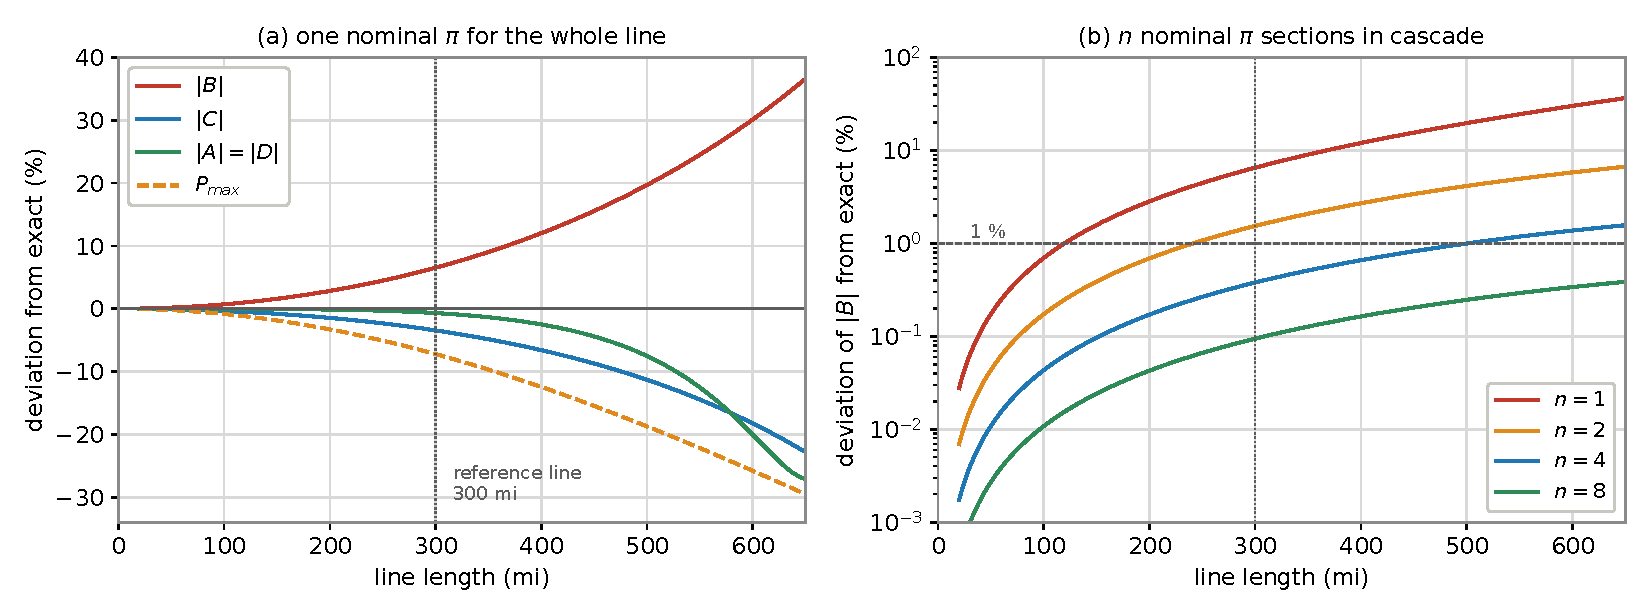
\includegraphics[width=\linewidth]{figures/ac/tp_model_error.pdf}
  \caption{(a) Deviation of the nominal $\pi$ against line length;
           (b) the same deviation of $\left|\underline{B}\right|$ when the
           line is built from $n$ cascaded $\pi$-sections. Both stop short
           of the quarter wavelength, where $\left|\underline{A}\right|$
           passes through zero}
  \label{fig:ref-model-error}
\end{figure}

\FloatBarrier

\subsubsection{Cascading shorter sections}
\label{sec:ref-cascade}

The nominal $\pi$ fails because one lumped section cannot represent a
distribution. The obvious repair is to use more of them: cut the line into
$n$ pieces of length $l/n$, model each as its own nominal $\pi$, and connect
the two-ports in cascade. The chain matrices multiply, so the whole line is
\begin{equation}
  \underline{T} = \left[\underline{T}_{\pi}
    \left(\frac{l}{n}\right)\right]^{n}
  \label{eq:ref-cascade}
\end{equation}
which is one matrix power, not $n$ separate models. Each section is shorter,
so each is a better approximation, and in the limit $n \to \infty$ the
product is the distributed solution of~\eqref{eq:ac-abcd-exact} --- the
cascade is how the exact form is reached from the lumped one.

Table~\ref{tab:ref-cascade} and Figure~\ref{fig:ref-model-error}(b) show the
convergence. The deviation falls with $1/n^2$ once the sections are
electrically short, so each doubling of $n$ buys a factor of four. What
governs the result is the electrical length of a \emph{section}, not of the
line: on this conductor, sections of about 100\,mi hold
$\left|\underline{B}\right|$ inside a percent at any total length, which is
the same 100\,mi that Table~\ref{tab:ref-pi-abs} gives for a whole line.

\begin{table}[!ht]
  \centering
  \begin{tabular}{@{}r l r r r r r@{}}
    \toprule
    \textbf{$n$} & \textbf{section}
      & \multicolumn{5}{c}{deviation of $\left|\underline{B}\right|$, \%} \\
    \cmidrule(lr){3-7}
    & & \multicolumn{1}{c}{100\,mi} & \multicolumn{1}{c}{200\,mi}
      & \multicolumn{1}{c}{300\,mi} & \multicolumn{1}{c}{400\,mi}
      & \multicolumn{1}{c}{600\,mi} \\
    \midrule
     1 & $l$      & $+0.70$ & $+2.83$ & $+6.53$ & $+12.03$ & $+30.13$ \\
     2 & $l/2$    & $+0.17$ & $+0.69$ & $+1.54$ &  $+2.71$ &  $+5.81$ \\
     4 & $l/4$    & $+0.04$ & $+0.17$ & $+0.38$ &  $+0.66$ &  $+1.38$ \\
     8 & $l/8$    & $+0.01$ & $+0.04$ & $+0.09$ &  $+0.16$ &  $+0.34$ \\
    16 & $l/16$   & $+0.00$ & $+0.01$ & $+0.02$ &  $+0.04$ &  $+0.08$ \\
    \bottomrule
  \end{tabular}
  \caption{Nominal $\pi$-sections in cascade: deviation of
           $\left|\underline{B}\right|$ from the exact two-port against the
           number of sections~[12]}
  \label{tab:ref-cascade}
\end{table}

Cascading is not the only repair, and for a plain line it is not the best
one. The equivalent $\pi$ of~\eqref{eq:ac-equivalent-pi} is exact with a
single section, and the correction it applies is not small: on this line at
300\,mi the series branch falls from $27.5 + j\,162.2\,\Omega$ to $24.1 +
j\,152.5\,\Omega$ and the shunt branch rises from 1.156 to 1.193\,mS at each
end, and at 600\,mi from $54.9 + j\,324.4$ to $30.4 + j\,251.0\,\Omega$
against 2.312 to 2.650\,mS. One exact section beats sixteen approximate
ones and costs less to evaluate.

Cascading earns its place where the single equivalent $\pi$ cannot go.

\begin{itemize}
  \setlength{\itemsep}{0.35em}
  \item \textbf{Something is connected part-way along.} A midpoint series
        bank is a two-port cascaded between two half-lines,
        Section~\ref{sec:series-compensation}, and a tapped substation or a
        transposition point divides the line in the same way. The
        equivalent $\pi$ describes a line between its own two ends and
        nothing else.
  \item \textbf{Quantities along the line are wanted.} The voltage profiles
        of Section~\ref{sec:np-profile} are the intermediate port
        quantities of a cascade; a single two-port gives only its terminals.
  \item \textbf{The line is not uniform.} Different conductor, spacing or
        bundle over part of the route gives each part its own matrix, and
        the product handles it with no extra theory. The equivalent $\pi$
        assumes one $\underline{\gamma}$ and one $\underline{Z}_w$ over the
        whole length.
  \item \textbf{A time-domain or frequency-sweep model is wanted.} The
        cascade is a lumped circuit a simulator can integrate directly,
        which is why electromagnetic-transient models still use chained
        sections rather than a closed-form $\cosh$.
\end{itemize}

Where the line is uniform and only its terminals matter, the equivalent
$\pi$ is the right model, and the cascade is a way of understanding where it
comes from. Appendix~\ref{sec:tp-interconnection} sets the cascade beside
the other ways two-ports combine, which are not interchangeable with it.

\subsubsection{The three representations compared}
\label{sec:ref-models}

Table~\ref{tab:ref-models} evaluates the two-port parameters and the crest
of the power-angle curve for the same line under the three representations
of Section~\ref{sec:ac-transmission}. The simplification
of~\eqref{eq:ac-simple} moves the maximum from $81.0^\circ$ to $90^\circ$
and overstates it by 13\,\%; the nominal $\pi$ keeps the angle but
understates the maximum by 7\,\%, because its $\left|\underline{B}\right|$
is too large. At 300\,mi $\left|\underline{A}\right| = 0.82$, so the line is
already far from the single series impedance that~\eqref{eq:ac-simple}
assumes. The numbers follow from the model of
Section~\ref{sec:ac-transmission} implemented in~[11].

\begin{table}[!ht]
  \centering
  \begin{tabular}{@{}l r r r r@{}}
    \toprule
    \textbf{Model} & \multicolumn{1}{c}{\textbf{$\left|A\right|$}}
      & \multicolumn{1}{c}{\textbf{$\vartheta_B$}}
      & \multicolumn{1}{c}{\textbf{$\left|B\right|$}}
      & \multicolumn{1}{c}{\textbf{$P_{max}$}} \\
    & & \multicolumn{1}{c}{$^\circ$} & \multicolumn{1}{c}{$\Omega$}
      & \multicolumn{1}{c}{MW} \\
    \midrule
    Short, lossless & 1.000 & 90.0 & 162.2 & 1541 \\
    Nominal $\pi$   & 0.813 & 80.4 & 164.5 & 1266 \\
    Distributed     & 0.819 & 81.0 & 154.4 & 1364 \\
    \bottomrule
  \end{tabular}
  \caption{Two-port parameters and maximum transfer at 300\,mi, both
           terminals at 1.0\,p.u.}
  \label{tab:ref-models}
\end{table}

\subsubsection{The surrounding system}
\label{sec:ref-scr}

The reactance that appears in~\eqref{eq:ac-simple} is the whole path between
the two internal voltages, not the line:
\begin{equation}
  X_{tot} = X_{th\_s} + X_{tr\_s} + X' + X_{tr\_r} + X_{th\_r},
  \qquad
  X_{th} = \frac{U_n^2}{S_{sc}},
  \qquad
  \mathrm{SCR} = \frac{S_{sc}}{P_n}
  \label{eq:ref-xtot}
\end{equation}
with $X_{th}$ the Thevenin reactance of the system behind a terminal, $X_{tr}$
that of the transformer and $S_{sc}$ the short-circuit level there. Taking the
lossless $P_{max} = U_n^2 / X_{tot}$ with equal systems at both ends and the
transformers neglected, Table~\ref{tab:ref-scr} shows how much of the
capability belongs to the terminals rather than to the line.

\begin{table}[!ht]
  \centering
  \begin{tabular}{@{}l r r r@{}}
    \toprule
    \textbf{SCL, each end} & \multicolumn{1}{c}{\textbf{$X_{th}$}}
      & \multicolumn{1}{c}{\textbf{$X_{tot}$}}
      & \multicolumn{1}{c}{\textbf{$P_{max}$}} \\
    \multicolumn{1}{c}{GVA} & \multicolumn{1}{c}{$\Omega$}
      & \multicolumn{1}{c}{$\Omega$} & \multicolumn{1}{c}{MW} \\
    \midrule
    5      & 50.0 & 253.4 &  986 \\
    10     & 25.0 & 203.4 & 1229 \\
    20     & 12.5 & 178.4 & 1401 \\
    stiff  &  0.0 & 153.4 & 1630 \\
    \bottomrule
  \end{tabular}
  \caption{Effect of the surrounding system on the maximum transfer of the
           300\,mi reference line, $X' = 153.4\,\Omega$, transformers
           neglected}
  \label{tab:ref-scr}
\end{table}

A quarter of the capability of this line into 10\,GVA systems is lost to the
terminals rather than to the line itself, which is why a loadability figure
quoted for a line in isolation is optimistic. The same quantity, normalised
as the short-circuit ratio, is what governs converter performance on a DC
link.

\subsubsection{What this is not}
\label{sec:ref-caveat}

$P_{max}$ is not a transfer capability. It is the crest of the power-angle
curve of an uncompensated line between two stiff systems, reached at an
angle no system is operated at. What the line can actually carry follows
from the thermal rating of the conductors, the permissible voltage drop and
the angular stability margin, and from the contingency case rather than the
intact one. Those limits are the subject of a separate section; the
representation of Section~\ref{sec:ac-transmission} is what they are
evaluated on.

\FloatBarrier

% =============================================================
%  Natural power (surge-impedance loading)
%  Figures copied from presentation/design/ac-transmission/fig/
%  (np_*.pdf), generated by that folder's natural_power_figures.py
%  from the exact two-port equations and cross-checked against a
%  20-segment pandapower model (deviation < 0.1 %).
%  Worked line of this section: 400 kV, 2x bundle, 50 Hz, 400 km --
%  not the 500 kV line of Section 6.
% =============================================================
\subsection{Natural Power}
\label{sec:natural-power}

\subsubsection{Definition}
\label{sec:np-definition}

A line terminated in its own wave impedance carries its \emph{natural
power}: the reactive power generated by the shunt capacitance exactly
cancels the reactive power consumed by the series inductance, the line
exchanges no reactive power with either end, and its voltage magnitude stays
constant along the route. North American practice calls the same quantity
the surge-impedance loading, SIL.

On an overhead line $\omega \cdot L' \gg R'$ and $\omega \cdot C' \gg G'$,
so the wave impedance of~\eqref{eq:ac-gamma-zw} is within about a percent of
the real quantity $\sqrt{L'/C'}$, and it is that real value the natural
power is quoted from:
\begin{equation}
  Z_w \approx \sqrt{\frac{L'}{C'}}
  \qquad
  P_{nat} = \mathrm{SIL} = \frac{U^2}{Z_w}
  \label{eq:np-definition}
\end{equation}

$Z_w$ is a property of the conductor geometry alone. It does not depend on
the length of the line, and in the lossless form not on frequency either.
$P_{nat}$ is therefore a reference rather than a rating: below it the line
is a net source of reactive power, above it a net sink.

The same result follows from the two-port equations. Closing the line with
$\underline{Z}_w$ makes $\underline{I}_R = \underline{U}_R /
\underline{Z}_w$, and~\eqref{eq:ac-u-x} and~\eqref{eq:ac-i-x} collapse to a
single travelling wave with no reflection,
\begin{equation}
  \underline{U}(x) = \underline{U}_R \cdot
      e^{\underline{\gamma} \cdot x},
  \qquad
  \underline{I}(x) = \underline{I}_R \cdot
      e^{\underline{\gamma} \cdot x}
  \label{eq:np-matched}
\end{equation}
so that $\underline{U}/\underline{I} = \underline{Z}_w$ everywhere and the
magnitude falls only by the attenuation $e^{-\alpha \cdot l}$,
Figure~\ref{fig:np-matched}. Only the complex $\underline{Z}_w$ matches
perfectly; terminating in the real $\sqrt{L'/C'}$ leaves a small residual
reflection.

\begin{figure}[!ht]
  \centering
  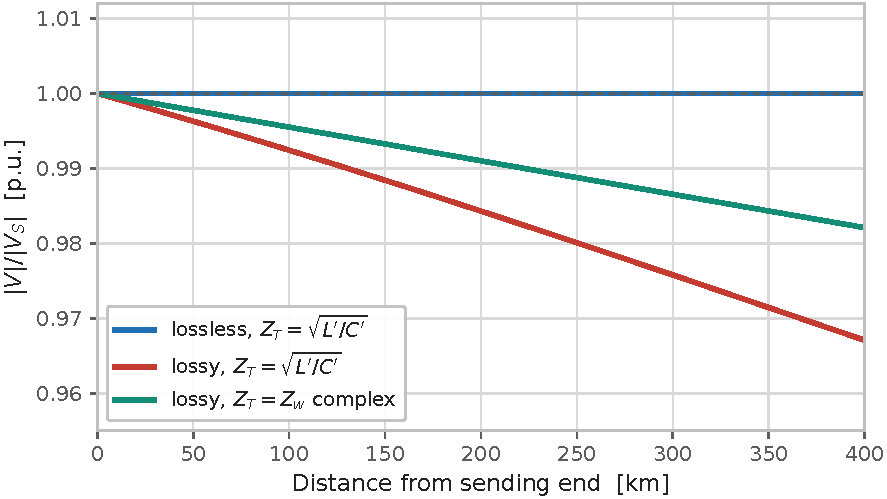
\includegraphics[width=0.78\linewidth]{figures/ac/np_matched_profile.pdf}
  \caption{Voltage along a line closed in its wave impedance: the profile is
           flat apart from the attenuation, and the residual ripple of the
           real-valued termination}
  \label{fig:np-matched}
\end{figure}

\subsubsection{The reactive balance}
\label{sec:np-balance}

Read as a reactive power balance, a line of length $l$ at line-to-line
voltage $U$ carrying phase current $I$ generates and consumes
\begin{equation}
  Q_C = \omega \cdot C' \cdot l \cdot U^2
  \qquad
  Q_L = 3 \cdot \omega \cdot L' \cdot l \cdot I^2
  \label{eq:np-qcql}
\end{equation}
Natural loading is where the two cancel. Setting $Q_C = Q_L$ eliminates both
$l$ and $\omega$ and gives $I = U / \left(\sqrt{3} \cdot Z_w\right)$, hence
$P_{nat} = \sqrt{3} \cdot U \cdot I = U^2 / Z_w$ again. The cancellation is
independent of length, which is why the natural power is a property of the
cross-section and not of the route.

The worked line of this section is a 400\,kV, 50\,Hz line of 400\,km with a
two-conductor bundle, $R' = 25$\,m$\Omega$/km, $X' = 0.30\,\Omega$/km and
$C' = 12.5$\,nF/km, giving $L' = 0.955$\,mH/km, $Z_w = 276.4\,\Omega$,
$\left|\underline{Z}_w\right| = 276.9\,\Omega$, $\beta \cdot l = 24.88^\circ$
and $P_{nat} = 579$\,MW. It is not the 500\,kV line of
Section~\ref{sec:reference-line}.

Losses move the balance. On the lossless line the zero crossing of the net
reactive flow reproduces $U^2 / Z_w$ to six decimals; on the real line it
falls to 566\,MW, 2.2\,\% below. The sending-end current carries the load
plus the losses, so $3 \cdot I^2 \cdot X' \cdot l$ is larger and the balance
is reached at a lower transfer. Figure~\ref{fig:np-balance} plots the net
reactive flow of both against the transfer.

\begin{figure}[!ht]
  \centering
  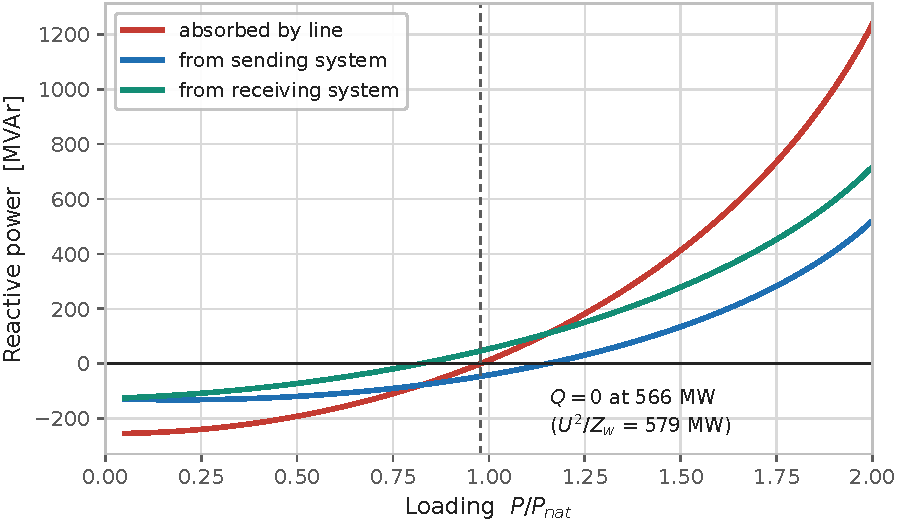
\includegraphics[width=0.78\linewidth]{figures/ac/np_reactive_balance.pdf}
  \caption{Net reactive power absorbed by the line against transfer,
           $Q_{line} = \Im\left\{\underline{S}_S\right\} -
           \Im\left\{\underline{S}_R\right\}$, lossless and real line}
  \label{fig:np-balance}
\end{figure}

\subsubsection{Voltage profile}
\label{sec:np-profile}

With both terminals held at 1.0\,p.u.\ and the transmission angle solved for
each loading, the profile along the line shows the balance directly,
Figure~\ref{fig:np-profile}. Below $P_{nat}$ the shunt capacitance dominates
and the middle of the line rises, to 1.024\,p.u.\ at no load. At $P_{nat}$
the profile is flat to four decimals. Above it the series reactance
dominates and the middle sags, to 0.873\,p.u.\ at $2 \cdot P_{nat}$, by
which point the angle across the line has reached $63^\circ$.

\begin{figure}[!ht]
  \centering
  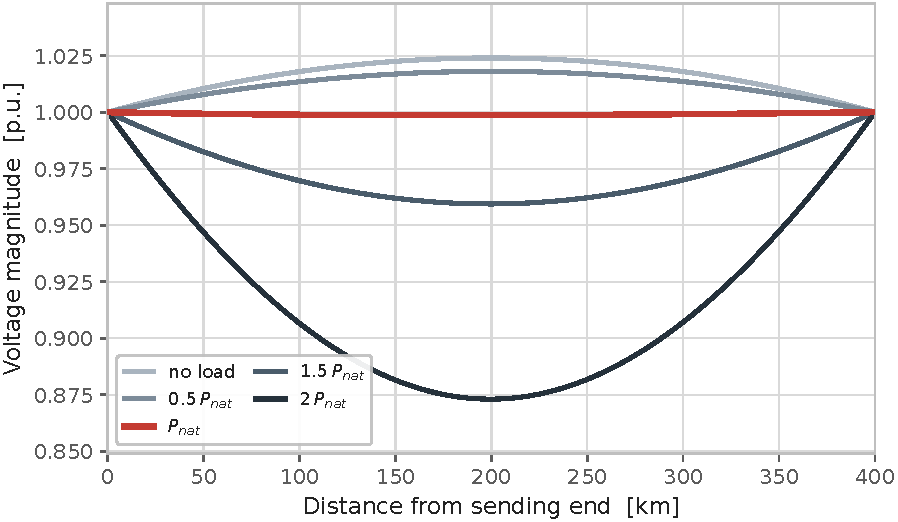
\includegraphics[width=0.78\linewidth]{figures/ac/np_voltage_profile.pdf}
  \caption{Voltage profile along the 400\,km line at several loadings, both
           terminals at 1.0\,p.u.}
  \label{fig:np-profile}
\end{figure}

\FloatBarrier

\subsubsection{Typical values}
\label{sec:np-typical}

Table~\ref{tab:np-typical} gives the natural power of common line types.

\begin{table}[!ht]
  \centering
  \begin{tabular}{@{}l r r r r r@{}}
    \toprule
    \textbf{Line} & \multicolumn{1}{c}{\textbf{$U$}}
      & \multicolumn{1}{c}{\textbf{$C'$}}
      & \multicolumn{1}{c}{\textbf{$Z_w$}}
      & \multicolumn{1}{c}{\textbf{$P_{nat}$}}
      & \multicolumn{1}{c}{\textbf{$S_{th}/P_{nat}$}} \\
    & \multicolumn{1}{c}{kV} & \multicolumn{1}{c}{nF/km}
      & \multicolumn{1}{c}{$\Omega$} & \multicolumn{1}{c}{MW} & \\
    \midrule
    230\,kV, $1\times$ Drake  & 230 &  9.0 & 376.1 &  141 & 2.8 \\
    345\,kV, $2\times$ bundle & 345 & 11.8 & 292.3 &  407 & 2.6 \\
    400\,kV, $2\times$ bundle & 400 & 12.5 & 276.4 &  579 & 2.4 \\
    500\,kV, $3\times$ bundle & 500 & 13.5 & 256.6 &  974 & 2.3 \\
    765\,kV, $4\times$ bundle & 765 & 13.5 & 250.8 & 2334 & 2.0 \\
    \bottomrule
  \end{tabular}
  \caption{Natural power of typical line types}
  \label{tab:np-typical}
\end{table}

Three things follow. $Z_w$ spans only 251 to 376\,$\Omega$ across the whole
range while $P_{nat}$ spans 141 to 2334\,MW, because $P_{nat}$ is a $U^2$
quantity: voltage, not geometry, is what buys transfer. Bundling and tighter
phase spacing are the only levers on $Z_w$, and they work on both terms, 
lowering $L'$ and raising $C'$. And the ratio of thermal rating to natural
power, $S_{th}/P_{nat}$, decides how far the thermal plateau of the
loadability curve of Section~\ref{sec:limits} extends.

AC cables sit at $Z_w \approx 20 \ldots 40\,\Omega$, so their natural power
is far above the thermal rating and never reached; as
Section~\ref{sec:cable} sets out, the charging current binds first.

\subsubsection{Light load: the Ferranti effect}
\label{sec:np-ferranti}

On an open-ended line $\underline{I}_R = 0$ and the terminal voltage ratio
follows from~\eqref{eq:ac-abcd-exact} as
\begin{equation}
  \frac{\underline{U}_R}{\underline{U}_S}
    = \frac{1}{\cosh\left(\underline{\gamma} \cdot l\right)}
    \;\longrightarrow\;
    \frac{1}{\cos\left(\beta \cdot l\right)}
  \label{eq:np-ferranti}
\end{equation}
in the lossless limit, so the receiving end rises above the sending end. At
$\beta \cdot l = 24.88^\circ$ the open end reaches 1.102\,p.u., drawing
251\,MVAr of charging power. A 60\,\% shunt reactor brings it back to
0.984\,p.u.; full compensation gives 0.918\,p.u., Figure~\ref{fig:np-ferranti}. The degree of compensation
follows from the light-load voltage, but it also moves the natural power.

\begin{figure}[!ht]
  \centering
  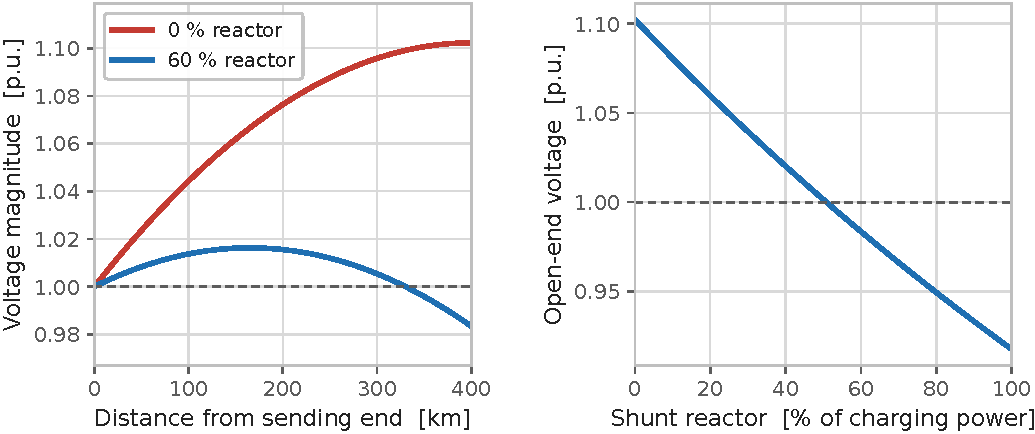
\includegraphics[width=0.74\linewidth]{figures/ac/np_ferranti.pdf}
  \caption{Open-end voltage rise against line length, and the effect of
           shunt compensation}
  \label{fig:np-ferranti}
\end{figure}

\subsubsection{Compensation moves the natural power}
\label{sec:np-compensation}

For uniformly distributed compensation the scaling is exact. Series
compensation of degree $k$ reduces the reactance and shunt compensation of
degree $m$ the capacitance:
\begin{equation}
  X' \to X' \cdot \left(1-k\right)
     \;\Rightarrow\; \frac{P_{nat}}{\sqrt{1-k}},
  \qquad
  C' \to C' \cdot \left(1-m\right)
     \;\Rightarrow\; P_{nat} \cdot \sqrt{1-m}
  \label{eq:np-compensation}
\end{equation}
so $k = 60$\,\% raises $P_{nat}$ by a factor 1.581 and $m = 60$\,\% lowers
it by 0.632, Figure~\ref{fig:np-compensation}.

Real banks are lumped at substations rather than distributed, so these laws
are a first-order guide only. A lumped 30\,\% series bank at $1.4 \cdot
P_{nat}$ on the worked line reduces the transmission angle from $37.6^\circ$
to $25.6^\circ$ and turns the sending-end reactive flow from $+89$ to
$-30$\,MVAr. Section~\ref{sec:series-compensation} treats the lumped case
properly.

\begin{figure}[!ht]
  \centering
  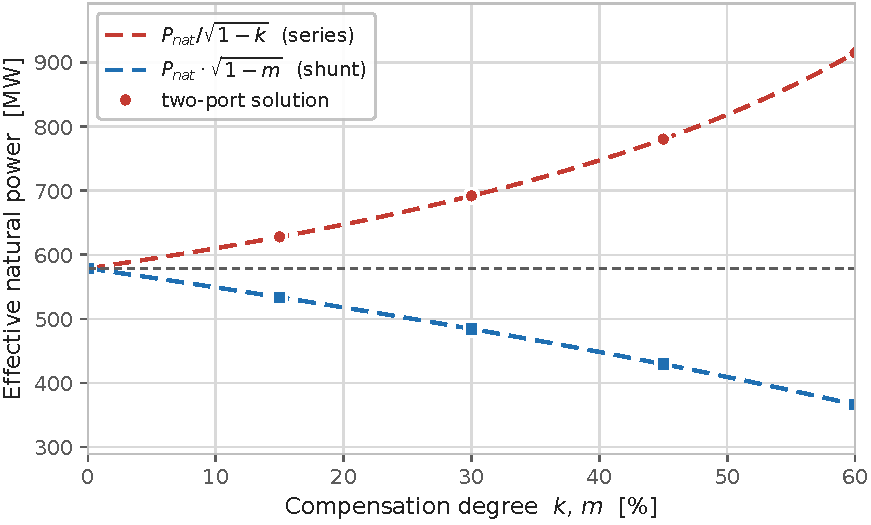
\includegraphics[width=0.74\linewidth]{figures/ac/np_compensation.pdf}
  \caption{Effect of distributed series and shunt compensation on the
           natural power}
  \label{fig:np-compensation}
\end{figure}

\FloatBarrier

% =============================================================
%  Transmission limits — thermal, voltage drop, angular stability
%  Figures copied from presentation/design/ac-transmission/fig/
%  (tl_*.pdf, np_loadability.pdf), generated by that folder's
%  transmission_limits_figures.py and natural_power_figures.py from
%  the exact two-port equations.
% =============================================================
\subsection{Transmission Limits}
\label{sec:limits}

The representation of Section~\ref{sec:ac-transmission} says what a line
does, not what it may be asked to do. Three criteria bound the transfer, and
which of them binds depends almost entirely on length.

\subsubsection{The three criteria}
\label{sec:limits-three}

\paragraph{Thermal.} The conductor temperature sets a current, and with it a
transfer that is independent of length:
\begin{equation}
  P_{th} = \sqrt{3} \cdot U_n \cdot I_{th}
  \label{eq:lim-thermal}
\end{equation}
The limiting mechanism is annealing of the aluminium and, more often, loss
of ground clearance through sag. It is the only one of the three that is a
property of the equipment rather than of the system, and it is weather- and
time-dependent, which is what dynamic line rating exploits.

\paragraph{Voltage drop.} The receiving-end voltage has to stay inside its
band under load. Written on the two-port,
\begin{equation}
  U_S = \left|\underline{A} \cdot \underline{U}_R
             + \underline{B} \cdot \underline{I}_R\right|
      \le 1.0\,\text{p.u.}
  \quad\text{with}\quad
  U_R \ge 0.95\,\text{p.u.}
  \label{eq:lim-voltage}
\end{equation}
Beyond natural loading the line is a net consumer of reactive power, and the
drop grows faster than the transfer. Shunt compensation at the receiving end
raises this limit at the cost of a weaker voltage-stability margin.

\paragraph{Steady-state stability.} The transmission angle must stay far
enough below the crest of the power-angle curve that the system survives the
loss of a parallel element. With a midpoint series bank of degree $k$ the
lossless form is
\begin{equation}
  P_{stab} \approx \frac{U^2}{\left(1-k\right) \cdot X_L}
            \cdot \sin\delta_{max}
  \label{eq:lim-stability}
\end{equation}
and a criterion of $\delta_{max} = 30^\circ$ leaves a factor two on the
lossless maximum. Section~\ref{sec:angular-stability} treats this limit
properly, including why the usable value is well below $P_{max}$.

The loadability of the line is the minimum of the three. Plotted against
length it is the St.~Clair curve.

\subsubsection{Loadability of the reference line}
\label{sec:limits-loadability}

Figure~\ref{fig:tl-loadability} evaluates the three criteria on the 500\,kV
reference line of Section~\ref{sec:reference-line} with the exact two-port
relations, for two boundary conditions. In case~(a) the load sits at the
receiving end with no reactive support, which is the classical St.~Clair
configuration. In case~(b) the line runs between two stiff systems with both
terminals held at 1.0\,p.u., which removes the voltage criterion entirely.
The thermal limit is $I_{th} = 3 \times 1300$\,A at 75\,$^\circ$C, giving
$P_{th} = 3377$\,MW against $P_{nat} = 939$\,MW.

\begin{figure}[!ht]
  \centering
  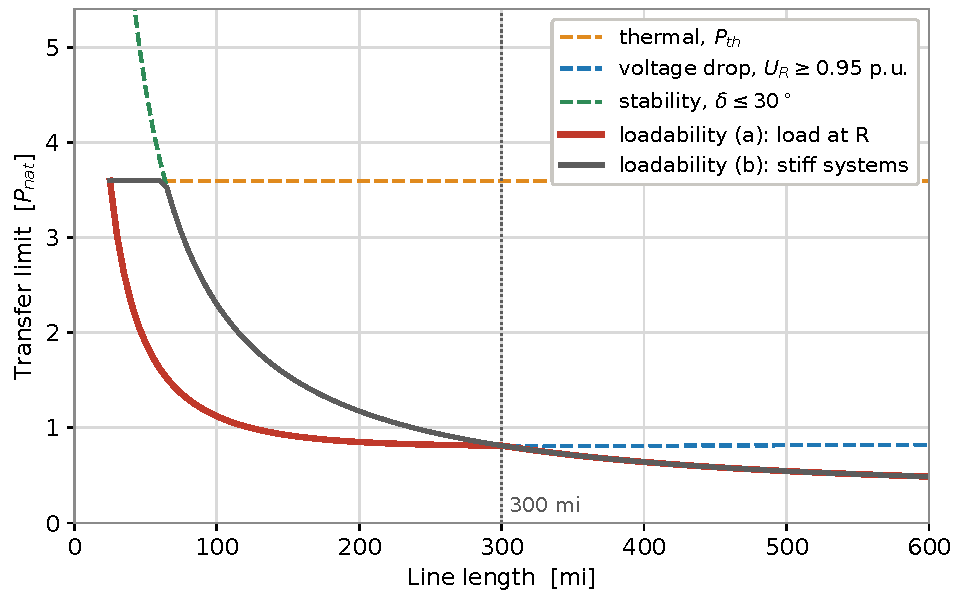
\includegraphics[width=0.78\linewidth]{figures/ac/tl_loadability.pdf}
  \caption{Loadability of the 500\,kV reference line against length, cases
           (a) and (b), uncompensated}
  \label{fig:tl-loadability}
\end{figure}

In case~(a) the thermal limit binds only to about 25\,mi, after which
voltage drop takes over, and the loadability falls through $1 \cdot P_{nat}$
at 125\,mi. In case~(b) the thermal limit holds to about 60\,mi and angular
stability binds beyond it, with the crossing at 240\,mi. At the 300\,mi
design length both cases give 763\,MW, or $0.81 \cdot P_{nat}$ --- the
voltage and the angle criterion happen to coincide there, and the line
cannot carry even its natural power without compensation.

The boundary condition is not a detail. Holding the receiving end at
1.0\,p.u.\ moves the $1 \cdot P_{nat}$ crossing by 115\,mi on this line. Any
loadability figure has to be quoted with the reactive support it assumes.

\subsubsection{The same analysis on the 400\,kV line}
\label{sec:limits-400}

Figure~\ref{fig:np-loadability} repeats the exercise on the 400\,kV, 50\,Hz
line of Section~\ref{sec:natural-power}, with criteria $I \le 2.0$\,kA,
$U_R \ge 0.95$\,p.u.\ and $\vartheta \le 30^\circ$. In case~(a) the thermal
limit holds to 80\,km at $2.3 \ldots 2.4 \cdot P_{nat}$, voltage drop binds
from 120 to 400\,km, angular stability beyond 500\,km, and the curve falls
through $1 \cdot P_{nat}$ at 382\,km. In case~(b) the thermal limit holds to
160\,km, stability binds beyond 200\,km, and the crossing moves to 472\,km.

\begin{figure}[!ht]
  \centering
  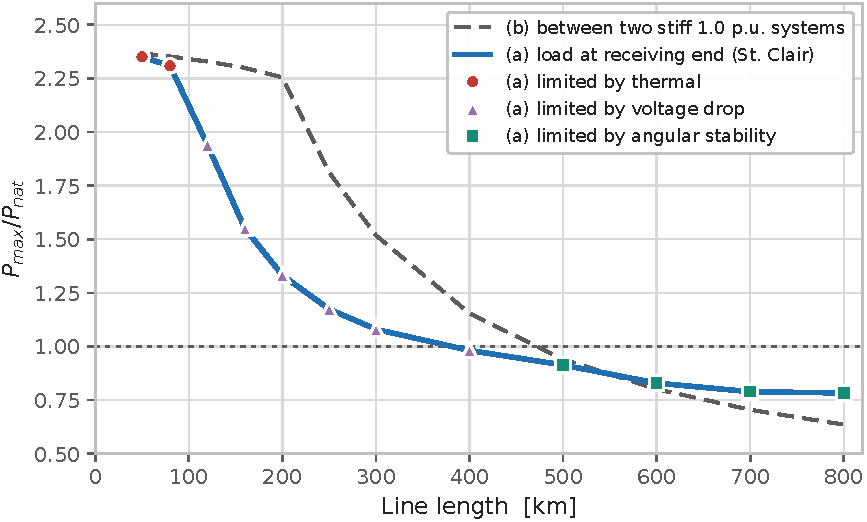
\includegraphics[width=0.78\linewidth]{figures/ac/np_loadability.pdf}
  \caption{Loadability of the 400\,kV line, showing that natural power is a
           reference and not a limit}
  \label{fig:np-loadability}
\end{figure}

The shape is the same on both lines: a thermal plateau of roughly $2 \ldots
2.5 \cdot P_{nat}$ over the first tens of kilometres, then a decay that
crosses natural power somewhere between a quarter and a half of a thousand
kilometres. That is the general statement the St.~Clair curve makes.

\FloatBarrier

\subsubsection{What compensation buys}
\label{sec:limits-compensation}

Figure~\ref{fig:tl-loadability-k} repeats case~(b) for a midpoint series
bank of degree $k$, and Table~\ref{tab:tl-k} gives the values at the 300\,mi
design length.

\begin{figure}[!ht]
  \centering
  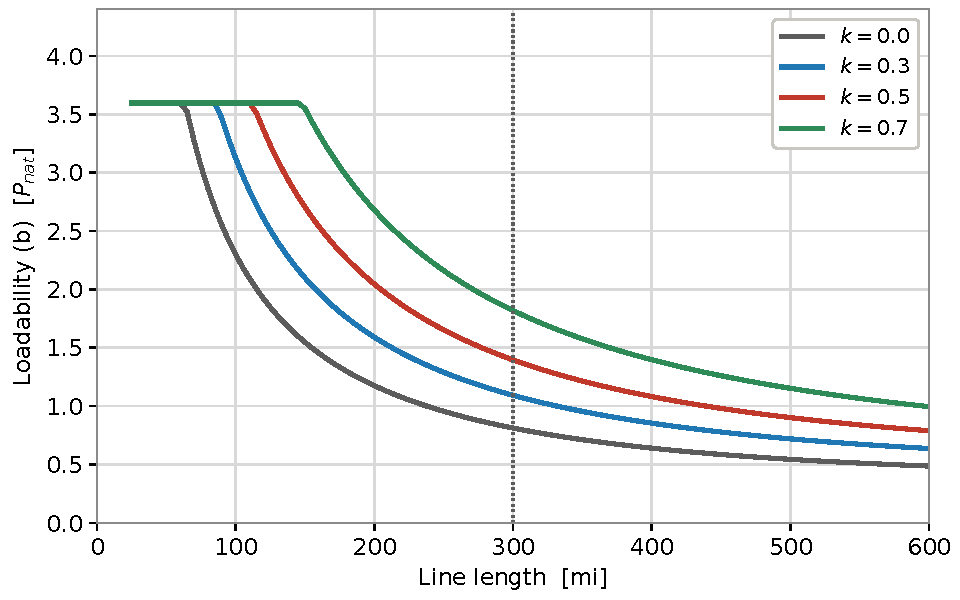
\includegraphics[width=0.74\linewidth]{figures/ac/tl_loadability_k.pdf}
  \caption{Case (b) loadability of the reference line with a midpoint series
           bank of degree $k$}
  \label{fig:tl-loadability-k}
\end{figure}

\begin{table}[!ht]
  \centering
  \begin{tabular}{@{}c r r r r@{}}
    \toprule
    \textbf{$k$} & \multicolumn{1}{c}{\textbf{$P_{stab}$}}
      & \multicolumn{1}{c}{\textbf{$P_U$}}
      & \multicolumn{1}{c}{\textbf{case (b)}}
      & \multicolumn{1}{c}{\textbf{thermal to}} \\
    & \multicolumn{1}{c}{MW} & \multicolumn{1}{c}{MW}
      & \multicolumn{1}{c}{$P_{nat}$} & \multicolumn{1}{c}{mi} \\
    \midrule
    0   &  763 & 763 & 0.81 &  60 \\
    0.3 & 1027 & 826 & 1.09 &  85 \\
    0.5 & 1311 & 844 & 1.40 & 110 \\
    0.7 & 1708 & 796 & 1.82 & 145 \\
    \bottomrule
  \end{tabular}
  \caption{Effect of a midpoint series bank at 300\,mi on the reference line}
  \label{tab:tl-k}
\end{table}

The bank acts on the stability limit: $k = 0.5$ lifts the 300\,mi
loadability of case~(b) from 0.81 to $1.40 \cdot P_{nat}$. The voltage limit
of case~(a) barely moves, because the $I \cdot X_C$ rise across the bank is
in quadrature with a unity-power-factor load. Series compensation therefore
does not remove the need for reactive support at the receiving end; it
addresses a different limit.

\subsubsection{Equipment limits}
\label{sec:limits-equipment}

The conductor is not always the first thing to run out. Currents follow from
the line-to-line voltage,
\begin{equation}
  I = \frac{S}{\sqrt{3} \cdot U_{LL}}
  \label{eq:lim-current}
\end{equation}
and the switchgear in series with the line carries the same current. The
largest continuous rating available in transmission circuit breakers is
about 5000\,A (Hitachi Energy, GE), so on a high-current scheme the breaker
rating, not the conductor, can set the maximum current and force either a
higher voltage or a second circuit.

\FloatBarrier

% =============================================================
%  Angular stability
%  Figures copied from presentation/design/ac-transmission/fig/
%  (as_*.pdf), generated by that folder's angular_stability_figures.py
%  from the exact two-port equations.  Worked line: the 500 kV
%  reference line of Section 6.
% =============================================================
\subsection{Angular Stability}
\label{sec:angular-stability}

Section~\ref{sec:limits} introduced the angular criterion as one of three
bounds. On any line long enough to matter it is the one that binds, and the
margin it needs is larger than the criterion alone suggests.

\subsubsection{Synchronising power}
\label{sec:as-ks}

The meaningful quantity is not the crest of the power-angle curve but its
slope, the \emph{synchronising power coefficient}
\begin{equation}
  K_s = \frac{\partial P}{\partial \delta}
      = \frac{U_S \cdot U_R}{X} \cdot \cos\delta
  \label{eq:as-ks}
\end{equation}
which is the stiffness of the electrical coupling between the machines at
either end. Below the maximum, a rotor that advances delivers more power,
decelerates and returns --- negative feedback. Beyond it, advancing delivers
less power and the machine accelerates further; $K_s = 0$ at the maximum is
therefore the steady-state stability limit in the strict sense.
Figure~\ref{fig:as-power-angle} shows both curves for the reference line.

\begin{figure}[!ht]
  \centering
  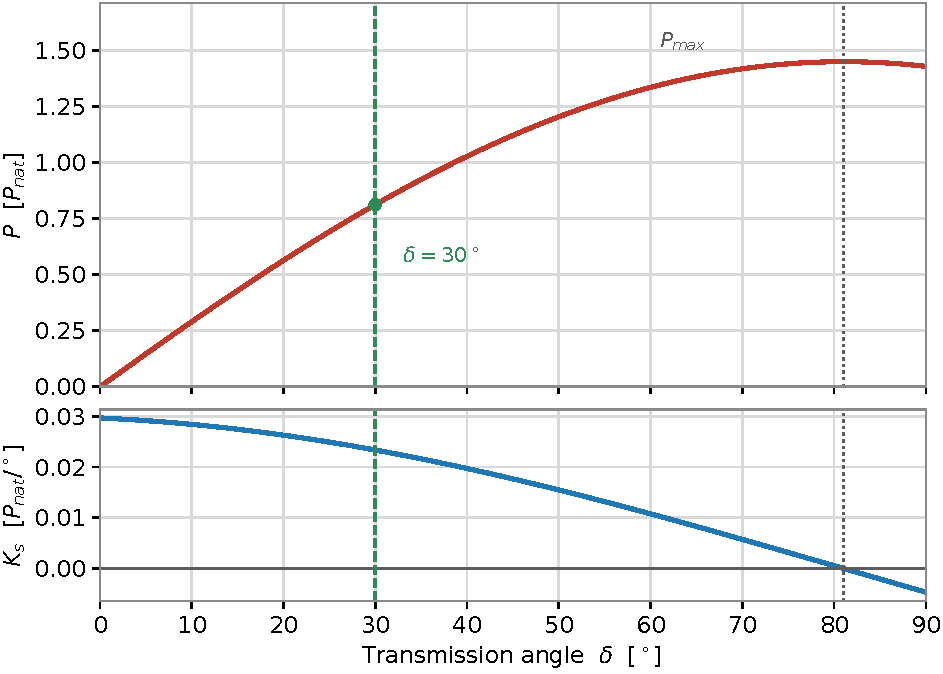
\includegraphics[width=0.74\linewidth]{figures/ac/as_power_angle.pdf}
  \caption{Power-angle relation and synchronising power coefficient of the
           500\,kV reference line at 300\,mi, both terminals at 1.0\,p.u.}
  \label{fig:as-power-angle}
\end{figure}

With losses the maximum does not fall at $90^\circ$ but at $\delta =
\vartheta_B$, which is $81.0^\circ$ on the reference line. At $\delta =
30^\circ$ the line carries $0.81 \cdot P_{nat}$ with 79\,\% of the stiffness
it has at $\delta = 0$.

Linearising the swing equation about an operating point gives
\begin{equation}
  \frac{2 \cdot H}{\omega_0} \cdot \Delta\ddot{\delta}
  + K_D \cdot \Delta\dot{\delta}
  + K_s \cdot \Delta\delta = 0
  \qquad
  \omega_n = \sqrt{\frac{K_s \cdot \omega_0}{2 \cdot H}}
  \label{eq:as-swing}
\end{equation}
with $H$ the inertia constant and $K_D$ the damping torque coefficient. As
$\delta$ grows, $K_s$ falls, the electromechanical mode slows and its
damping ratio drops. The machine becomes sluggish and poorly damped well
before it actually pulls out, which is the real reason nobody operates near
the maximum.

\subsubsection{Electrical length}
\label{sec:as-electrical-length}

For anything over roughly 250\,km the lumped $\omega \cdot L' \cdot l$
overstates the reactance. The series element of the exact equivalent is
$X' = Z_w \cdot \sin\left(\beta \cdot l\right)$, and substituting into the
lossless maximum gives a clean result:
\begin{equation}
  P_{max} = \frac{U^2}{Z_w \cdot \sin\left(\beta \cdot l\right)}
          = \frac{P_{nat}}{\sin\left(\beta \cdot l\right)}
  \label{eq:as-electrical-length}
\end{equation}
At a quarter wavelength --- 1234\,km on the reference line at 60\,Hz --- the
maximum transfer is exactly $P_{nat}$. That is the analytical spine beneath
the St.~Clair curve, and the reason capability decays with length rather
than staying flat. Figure~\ref{fig:as-electrical-length} compares the three
against length.

\begin{figure}[!ht]
  \centering
  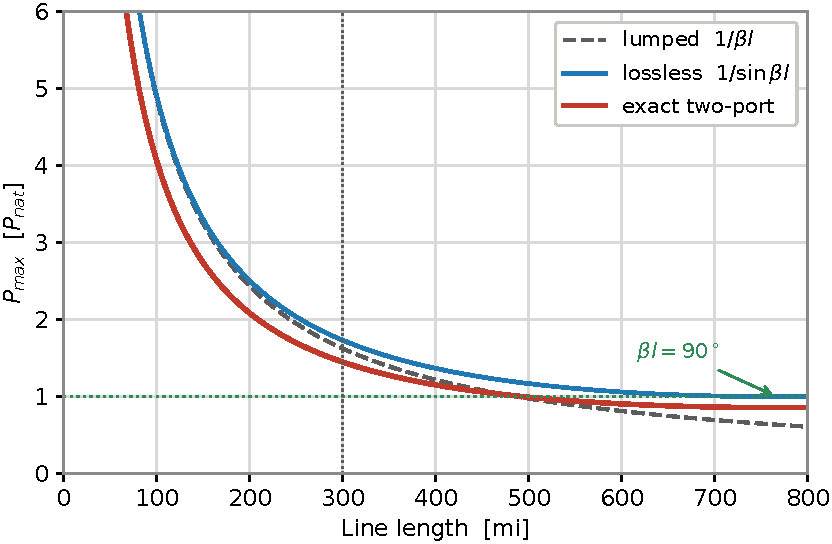
\includegraphics[width=0.74\linewidth]{figures/ac/as_electrical_length.pdf}
  \caption{Maximum transfer against length: lumped, lossless distributed and
           exact two-port}
  \label{fig:as-electrical-length}
\end{figure}

At the 300\,mi design length $\beta \cdot l = 35.2^\circ$, the lumped
reactance is $162.4\,\Omega$ against $X' = 153.4\,\Omega$, and
$1/\sin\left(\beta \cdot l\right) = 1.73$ against 1.45 for the exact
two-port; losses and charging account for the remaining gap.

\FloatBarrier

\subsubsection{From the maximum to the operating limit}
\label{sec:as-contingency}

Two effects cut the usable transfer well below $P_{max}$, and they compound.

The first is the post-contingency network. Two parallel 300\,mi circuits
have $P_{max} = 2726$\,MW intact; losing one doubles the reactance of the
path and leaves 1363\,MW on the survivor. Planning practice requires a
margin of 30 to 35\,\% on the \emph{post-contingency} network,
\begin{equation}
  \frac{P_{max} - P}{P_{max}} \ge 0.30
  \label{eq:as-margin}
\end{equation}
which on this pair allows 954\,MW, or $1.02 \cdot P_{nat}$ for the two
circuits together. A transfer of 1200\,MW looks comfortable intact, at
$\delta = 22.9^\circ$, and sits only 12\,\% below the post-contingency
maximum --- not acceptable. For comparison, the thermal rating of the pair
is 6755\,MW, seven times the binding constraint.
Figure~\ref{fig:as-contingency} shows both power-angle curves.

\begin{figure}[!ht]
  \centering
  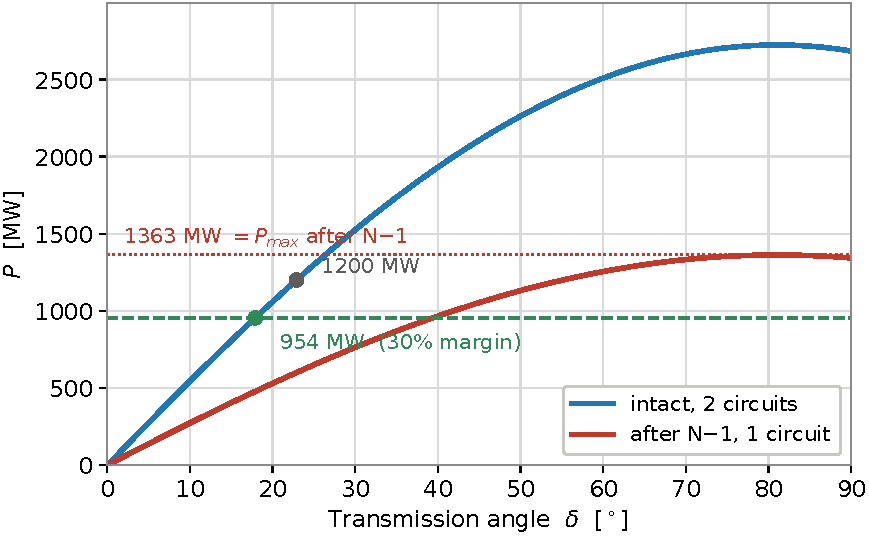
\includegraphics[width=0.74\linewidth]{figures/ac/as_contingency.pdf}
  \caption{Power-angle curves of two parallel 300\,mi circuits, intact and
           after the loss of one}
  \label{fig:as-contingency}
\end{figure}

\subsubsection{Transient stability}
\label{sec:as-equal-area}

The second effect is the fault case. During a fault the electrical output
collapses while the mechanical input continues; the rotor must give that
energy back before the maximum angle is reached. The equal-area criterion
states the condition as
\begin{equation}
  A_{acc} = \int_{\delta_0}^{\delta_{cc}}
            \left(P_m - P_{flt}\right) \mathrm{d}\delta
  \;=\;
  A_{dec} = \int_{\delta_{cc}}^{\delta_{max}}
            \left(P_{pst} - P_m\right) \mathrm{d}\delta
  \label{eq:as-equal-area}
\end{equation}
with $\delta_{cc}$ the clearing angle. For a machine at $P_m = 0.6$\,p.u.\
with maxima of 1.0 pre-fault, 0.3 during the fault and 0.7 after it,
$\delta_0 = 36.9^\circ$, $\delta_{cc} = 45.5^\circ$ and $\delta_{max} =
121.0^\circ$, Figure~\ref{fig:as-equal-area}.

\begin{figure}[!ht]
  \centering
  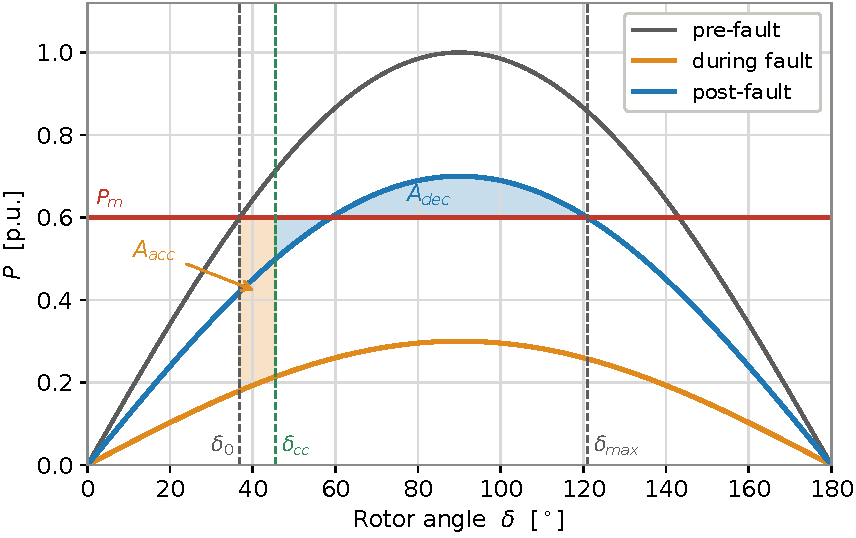
\includegraphics[width=0.72\linewidth]{figures/ac/as_equal_area.pdf}
  \caption{Equal-area criterion, generic machine per unit}
  \label{fig:as-equal-area}
\end{figure}

A higher pre-fault angle shrinks the decelerating area from both ends at
once, so the critical clearing time falls steeply with loading. This is why
two-cycle breakers and independent-pole tripping buy transfer capability,
and why the transient limit usually binds before the steady-state one.

\FloatBarrier

\subsubsection{Damping}
\label{sec:as-damping}

In a multi-machine system the classical limit generalises to an eigenvalue
criterion. The modes that constrain long transfers are the inter-area modes
at 0.2 to 0.8\,Hz; local plant modes sit at 0.8 to 2\,Hz and torsional modes
far above. The practical limit is where the damping ratio of a critical mode
falls below about 3 to 5\,\%, which can occur at angles well under
$40^\circ$ and therefore well below the two-machine maximum.

High-gain automatic voltage regulators, which are what allow a large angle
in the first place, contribute \emph{negative} damping torque at heavy
loading. The power system stabiliser exists to put it back. Tuning it, not
raising $P_{max}$, is often what releases transfer on a long corridor.

\subsubsection{Why a DC link has none of this}
\label{sec:as-dc}

A DC link has no transmission angle, no synchronising torque and no
equal-area criterion. The converter control sets power as a commanded
quantity, and length enters only through the conductor resistance, so the
$1/\sin\left(\beta \cdot l\right)$ decay of~\eqref{eq:as-electrical-length}
has no counterpart. An embedded DC link can be modulated to damp the
inter-area modes of the surrounding AC system instead of loading them.

The constraint moves to the terminals: short-circuit ratio and commutation
robustness for line-commutated converters, control interaction for
voltage-sourced ones. That is the trade the rest of this report is about.

\FloatBarrier

% =============================================================
%  Series compensation
%  Figures copied from presentation/design/ac-transmission/fig/
%  (sc_*.pdf), generated by that folder's series_compensation_figures.py
%  from the exact two-port equations with the bank cascaded as a
%  series element.  Worked line: the 500 kV reference line of Section 6.
% =============================================================
\subsection{Series Compensation}
\label{sec:series-compensation}

\subsubsection{Principle}
\label{sec:sc-principle}

A capacitor bank in series with the line cancels part of its inductive
reactance. The degree of compensation is defined against the total series
reactance,
\begin{equation}
  k = \frac{X_C}{X_L},
  \qquad X_L = \omega \cdot L' \cdot l,
  \qquad X_{eff} = \left(1-k\right) \cdot X_L
  \label{eq:sc-k}
\end{equation}
so that the lossless transfer becomes
\begin{equation}
  P = \frac{U^2}{\left(1-k\right) \cdot X_L} \cdot \sin\delta
  \label{eq:sc-power}
\end{equation}
with $\left|U_S\right| = \left|U_R\right| = U$. The line behaves as though
it were shorter: for a given transfer the angle falls and the stability
margin of Section~\ref{sec:angular-stability} rises.

Two properties distinguish it from shunt compensation. The voltage rise
$I \cdot X_C$ across the bank scales with the current, so the compensation
is self-regulating: it appears when it is needed and not at light load. And
it acts on the series branch, which is why it addresses the angular limit
and barely moves the voltage limit of case~(a) in
Section~\ref{sec:limits-compensation}.

The practical range is $k \approx 0.25 \ldots 0.70$. Above that,
sub-synchronous resonance, distance-protection behaviour and bank cost
dominate the choice.

In the two-port model the bank is cascaded as a series element at the point
where it is installed,
\begin{equation}
  \begin{bmatrix} 1 & -j \cdot X_C \\ 0 & 1 \end{bmatrix}
  \label{eq:sc-twoport}
\end{equation}
between the two half-lines for a midpoint bank, which is the arrangement
used throughout this section.

\subsubsection{Single-line arrangement}
\label{sec:sc-sld}

A series bank is not only capacitors. The platform sits at line potential
and carries the full fault current until it is bypassed, so each phase
carries a metal-oxide varistor across the bank to limit the capacitor
voltage under fault current, a bypass breaker with a damping reactor to take
over when the varistor reaches its energy limit, and disconnectors to
isolate the platform. A bypass disconnector keeps the line in service with
the bank out, at $k = 0$. Figure~\ref{fig:sc-sld} shows the arrangement for
one phase, with the bank at the midpoint of the line.

\begin{figure}[!ht]
  \centering
  \begin{tikzpicture}[x=1.07mm, y=1.07mm,
      wire/.style={draw=atFg, line width=0.35mm, line cap=round, line join=round},
      hair/.style={draw=atFg, line width=0.22mm, line cap=round, line join=round},
      bus/.style={draw=atFg, line width=0.9mm, line cap=butt},
      lbl/.style={font=\footnotesize, atFg},
      sub/.style={font=\scriptsize, atFgMuted},
      dot/.style={fill=atFg, circle, inner sep=0pt, minimum size=1.1mm}]
    % buses and line
    \draw[bus] (0,-8) -- (0,8);     \node[lbl,above] at (0,8.5) {S};
    \draw[bus] (120,-8) -- (120,8); \node[lbl,above] at (120,8.5) {R};
    \draw[wire] (0,0) -- (30,0);
    \draw[wire] (90,0) -- (120,0);
    \node[sub] at (15,3.2) {$l/2$};
    \node[sub] at (105,3.2) {$l/2$};
    % line disconnectors into the platform
    \draw[wire] (30,0) -- (33,0);
    \draw[wire] (33,0) -- (38.5,3.5);
    \draw[wire] (39,0) -- (42,0);
    \node[sub,above] at (36,4) {DS1};
    \draw[wire] (78,0) -- (81,0);
    \draw[wire] (81,0) -- (86.5,3.5);
    \draw[wire] (87,0) -- (90,0);
    \node[sub,above] at (84,4) {DS2};
    % main branch: series capacitor
    \node[dot] at (42,0) {};  \node[dot] at (78,0) {};
    \draw[wire] (42,0) -- (57,0);
    \draw[wire] (57,-4) -- (57,4);  \draw[wire] (60,-4) -- (60,4);
    \draw[wire] (60,0) -- (78,0);
    \node[lbl,above] at (58.5,4.8) {$C$\quad{\scriptsize\color{atFgMuted}$X_C = k \cdot X_L$}};
    % MOV branch
    \draw[wire] (42,0) -- (42,-10) -- (54,-10);
    \draw[wire] (54,-13) rectangle (66,-7);
    \draw[hair] (55,-12) -- (65,-8);
    \draw[wire] (66,-10) -- (78,-10) -- (78,0);
    \node[sub,below] at (60,-13.3) {MOV};
    % damping reactor and bypass breaker
    \draw[wire] (42,-10) -- (42,-20) -- (50,-20);
    \draw[wire] (50,-22) rectangle (58,-18);
    \draw[wire] (58,-20) -- (63,-20);
    \draw[wire] (63,-22) -- (67,-18);  \draw[wire] (63,-18) -- (67,-22);
    \draw[wire] (67,-20) -- (78,-20) -- (78,-10);
    \node[sub,below] at (54,-22.3) {$L_d$};
    \node[sub,below] at (65,-22.3) {bypass CB};
    % bypass disconnector around the whole bank
    \draw[wire] (33,0) -- (33,-33) -- (55,-33);
    \draw[wire] (55,-33) -- (60.5,-29.5);
    \draw[wire] (61,-33) -- (87,-33) -- (87,0);
    \node[sub,below] at (58,-34) {bypass DS};
    % platform outline
    \draw[atFgMuted, line width=0.4pt, densely dashed] (39,-27.5) rectangle (81,12.5);
    \node[sub,anchor=south east] at (81,12.8) {capacitor platform, line potential};
    % current arrow
    \draw[-{Stealth[length=2mm]}, atFgMuted] (8,-3.5) -- (22,-3.5)
      node[midway,below,sub] {$I$};
  \end{tikzpicture}
  \caption{Single-line diagram of a midpoint series bank, one phase.
           Symbols to IEC 60617~[18]}
  \label{fig:sc-sld}
\end{figure}

The varistor limits the capacitor voltage under fault current and the bypass
breaker with its damping reactor $L_d$ takes over at the varistor energy
limit. DS1 and DS2 isolate the platform; the bypass disconnector keeps the
line in service with the bank out.

\subsubsection{Effect on the power-angle curve}
\label{sec:sc-power-angle}

Figure~\ref{fig:sc-power-angle} shows the power-angle curves of the 500\,kV
reference line for a midpoint bank at several degrees of compensation, and
Table~\ref{tab:sc-power-angle} the resulting maxima.

\begin{figure}[!ht]
  \centering
  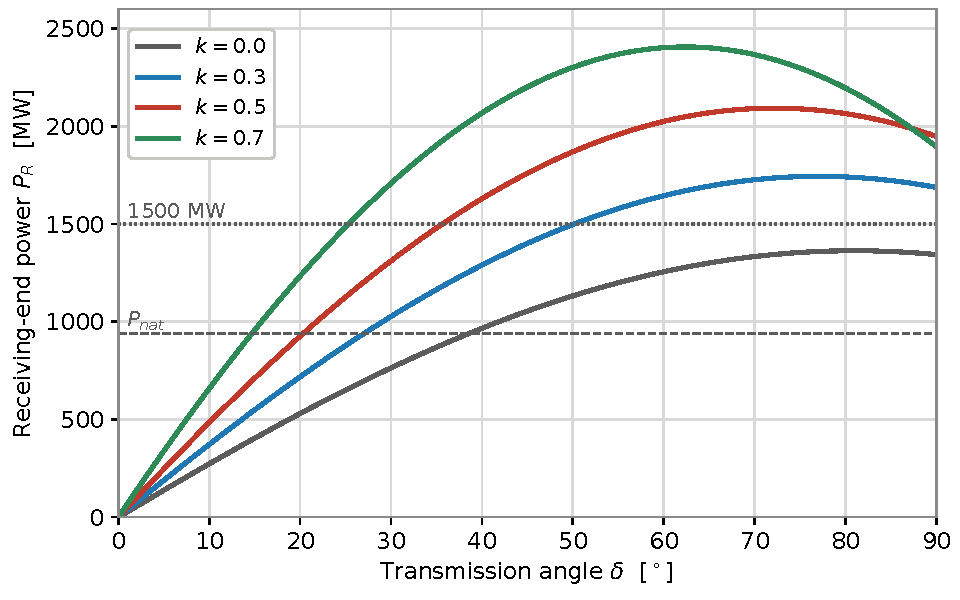
\includegraphics[width=0.74\linewidth]{figures/ac/sc_power_angle.pdf}
  \caption{Power-angle curves of the reference line with a midpoint series
           bank, both terminals at 1.0\,p.u.}
  \label{fig:sc-power-angle}
\end{figure}

\begin{table}[!ht]
  \centering
  \begin{tabular}{@{}c r r r@{}}
    \toprule
    \textbf{$k$} & \multicolumn{1}{c}{\textbf{$X_C$}}
      & \multicolumn{1}{c}{\textbf{$P_{max}$}}
      & \multicolumn{1}{c}{\textbf{$\delta$ at 1500\,MW}} \\
    & \multicolumn{1}{c}{$\Omega$} & \multicolumn{1}{c}{MW}
      & \multicolumn{1}{c}{$^\circ$} \\
    \midrule
    0   & 0     & 1363 & --- \\
    0.3 & 48.7  & 1744 & 50.1 \\
    0.5 & 81.2  & 2093 & 35.7 \\
    0.7 & 113.7 & 2407 & 25.3 \\
    \bottomrule
  \end{tabular}
  \caption{Midpoint bank on the 300\,mi reference line, exact two-port}
  \label{tab:sc-power-angle}
\end{table}

Uncompensated, 1500\,MW --- $1.6 \cdot P_{nat}$ --- cannot be carried at
all; at $k = 0.5$ it is carried at $36^\circ$. The maximum also moves to
smaller angles as $k$ grows, which is the electrical shortening of the line
expressed on the curve. The lossless form
$U^2 / \left(\left(1-k\right) \cdot X_L\right)$ would give 1540\,MW
uncompensated and 3080\,MW at $k = 0.5$; at this length $R = 27.5\,\Omega$
and the line charging are not negligible, which is why the exact two-port is
used.

\subsubsection{Voltage profile at heavy load}
\label{sec:sc-voltage}

Delivering 900\,MW at $\cos\varphi = 0.95$ lagging with the receiving end
held at 1.0\,p.u., the uncompensated line requires a sending-end voltage of
1.217\,p.u., far outside any operating band. The midpoint bank lifts the
voltage by $I \cdot X_C$ in the direction of power flow, and the sending end
falls to 1.157, 1.127 and 1.107\,p.u.\ for $k = 0.3$, 0.5 and 0.7,
Figure~\ref{fig:sc-voltage}.

\begin{figure}[!ht]
  \centering
  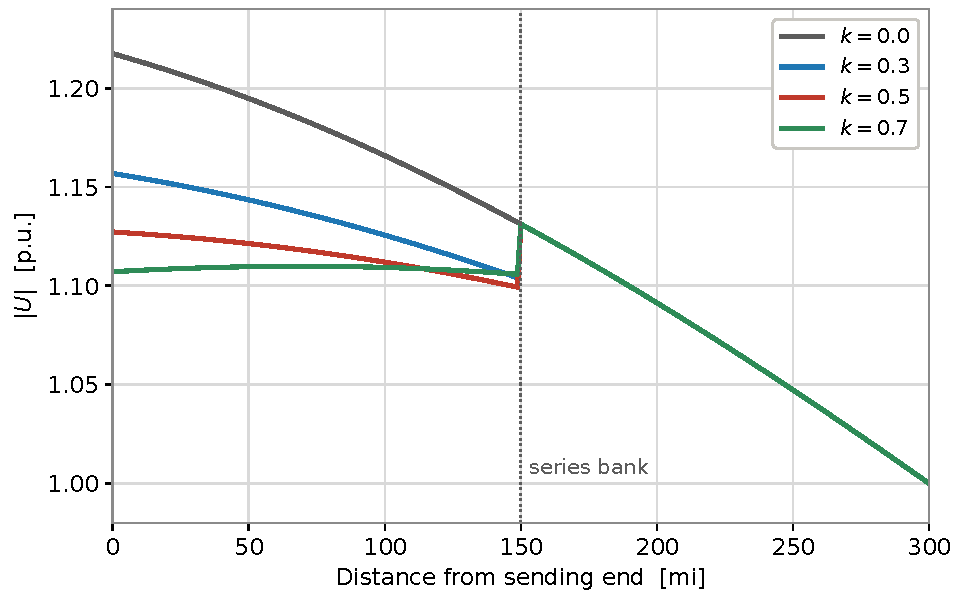
\includegraphics[width=0.74\linewidth]{figures/ac/sc_voltage_profile.pdf}
  \caption{Voltage profile at heavy load with a midpoint series bank}
  \label{fig:sc-voltage}
\end{figure}

The receiving half of the line is unchanged, because the bank acts only on
what is upstream of it. That is why end-of-line banks and split banks are
also used where the voltage profile rather than the angle is the problem.

\FloatBarrier

\subsubsection{Bank rating and protection}
\label{sec:sc-rating}

The bank is rated for the planned continuous line current, not for the
conductor thermal limit:
\begin{equation}
  U_C = I_{rated} \cdot X_C
  \qquad
  Q_C = 3 \cdot I_{rated}^{2} \cdot X_C
  \label{eq:sc-rating}
\end{equation}
Table~\ref{tab:sc-rating} gives the resulting bank for the reference line at
$k = 0.5$.

\begin{table}[!ht]
  \centering
  \begin{tabular}{@{}l l r@{}}
    \toprule
    \textbf{Quantity} & & \multicolumn{1}{c}{\textbf{Value}} \\
    \midrule
    $k$ & & 0.5 \\
    $X_C$ & $\Omega$ & 81.2 \\
    $C$ per phase & \textmu F & 32.7 \\
    $I_{rated}$ & A & 2000 \\
    \midrule
    $U_C$ per phase & kV & 162 \\
    $Q_C$ three-phase & MVAr & 974 \\
    MOV level ($2.3 \cdot U_C$) & kV & 373 \\
    \bottomrule
  \end{tabular}
  \caption{Midpoint bank rating on the reference line at $k = 0.5$}
  \label{tab:sc-rating}
\end{table}

$I_{rated}$ is taken as about $1.15 \cdot$ the current at 1500\,MW and
500\,kV. The fault-current voltage is limited by the metal-oxide varistor at
a protective level of $2.0 \ldots 2.5 \cdot U_C$, with the bypass breaker
and damping circuit behind it. Emergency ratings --- typically 30\,min and
10\,s --- are specified separately from the continuous rating.

\subsubsection{Sub-synchronous resonance}
\label{sec:sc-ssr}

The bank forms a series resonance with the line and source reactances at
\begin{equation}
  f_{er} = f_0 \cdot \sqrt{\frac{X_C}{X_L + X_S}}
  \label{eq:sc-ssr}
\end{equation}
Rotor currents see the complement $f_0 - f_{er}$, which has to stay clear of
the torsional modes of the turbine-generator shaft --- 10 to 45\,Hz for
large steam units. Figure~\ref{fig:sc-ssr} screens the reference line against
the degree of compensation.

\begin{figure}[!ht]
  \centering
  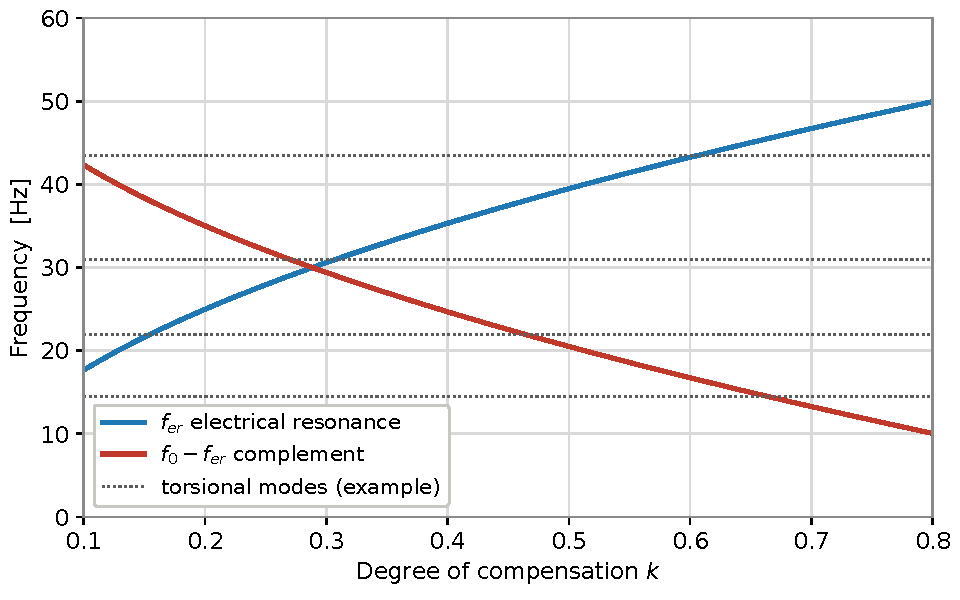
\includegraphics[width=0.72\linewidth]{figures/ac/sc_ssr_screening.pdf}
  \caption{Sub-synchronous resonance screening: electrical resonance and its
           complement against the degree of compensation}
  \label{fig:sc-ssr}
\end{figure}

With $X_S = 25\,\Omega$, which is 15\,\% on 1500\,MVA, a compensation of
$k = 0.5$ gives $f_{er} = 39.5$\,Hz and a complement of 20.5\,Hz --- within
2\,Hz of an illustrative 22\,Hz torsional mode. A hit at screening level
calls for a detailed study or a different $k$; type-3 wind generation adds
sub-synchronous control interaction to the same screening. The torsional
modes used at this stage are illustrative, and real values come from the
generator manufacturer.

\FloatBarrier

\section{References}
\label{sec:references}

\begin{enumerate}[label={[\arabic*]}, leftmargin=*, itemsep=0.4em]
  \item IEC TS 60815-4:2016, \emph{Selection and dimensioning of high-voltage
        insulators intended for use in polluted conditions --- Part 4:
        Insulators for d.c.\ systems}.
  \item CIGRE Working Group C4.303, TB 518, \emph{Outdoor insulation in
        polluted conditions: Guidelines for selection and dimensioning ---
        Part 2: The DC case}, 2012.
  \item CIGRE Working Group B4.45, TB 417, \emph{Technological Assessment of
        800\,kV HVDC Applications}, June 2010, Sections~7.1.8.3 ``Corrections for altitudes'' and
        12.1 ``Flashover process''.
  \item IEC TS 60815-1:2008, \emph{Selection and dimensioning of high-voltage
        insulators intended for use in polluted conditions --- Part 1:
        Definitions, information and general principles}.
  \item F.~Obenaus, ``Fremdschichtüberschlag und Kriechweglänge'',
        \emph{Deutsche Elektrotechnik}, vol.~4, pp.~135--136, 1958.
  \item B.~F.~Hampton, ``Flashover mechanism of polluted insulation'',
        \emph{Proceedings of the IEE}, vol.~111, no.~5, pp.~985--990, 1964.
  \item IEC 60507:2013, \emph{Artificial pollution tests on high-voltage
        ceramic and glass insulators to be used on a.c.\ systems}.
  \item CIGRE Working Group D1.44, TB 705, \emph{Guidelines for Altitude
        Correction of Pollution Performance of Insulators}, November 2017,
        Section~3.2 ``DC guidelines''.
  \item IEC 60071-2:2018, \emph{Insulation co-ordination --- Part 2:
        Application guidelines}.
  \item Southwire Company, \emph{ACSR --- Aluminum Conductor, Steel
        Reinforced, Bare}, catalog section 11-4,
        \path{southwire.com/wire-cable/bare-aluminum-overhead-transmission-distribution}.
  \item \emph{Two-port evaluation of the 500\,kV reference line} (numpy,
        exact and nominal-$\pi$ models),
        \path{presentation/design/ac-transmission/fig/angular_stability_figures.py}.
  \item \emph{Lumped and distributed two-port models of the 500\,kV reference
        line} (numpy, nominal $\pi$, cascaded sections and the exact form),
        \path{presentation/design/ac-transmission/fig/two_port_models.py}.
  \item ASTM B232/B232M, \emph{Standard Specification for Concentric-Lay-Stranded
        Aluminum Conductor, Steel-Reinforced (ACSR)}.
  \item ASTM B231/B231M, \emph{Standard Specification for Concentric-Lay-Stranded
        Aluminum 1350 Conductors}.
  \item ASTM B399/B399M, \emph{Standard Specification for Concentric-Lay-Stranded
        Aluminum Alloy 6201-T81 Conductors}.
  \item BS 215-2, \emph{Aluminium conductors and aluminium conductors,
        steel-reinforced, for overhead power transmission --- Part 2}.
  \item ABB, \emph{XLPE Submarine Cable Systems --- Attachment to XLPE Land
        Cable Systems User's Guide}, document 2GM5007, \path{new.abb.com}.
  \item IEC 60617, \emph{Graphical symbols for diagrams}.
  \item IEC 60050-131:2002, \emph{International Electrotechnical Vocabulary ---
        Part 131: Circuit theory}.
  \item L.~O.~Chua, C.~A.~Desoer and E.~S.~Kuh, \emph{Linear and Nonlinear
        Circuits}, McGraw-Hill, 1987, Chapter~17 ``Two-ports''.
  \item J.~J.~Grainger and W.~D.~Stevenson, \emph{Power System Analysis},
        McGraw-Hill, 1994, Chapter~6 ``Current and voltage relations on a
        transmission line''.
  \item L.~L.~Beranek and T.~J.~Mellow, \emph{Acoustics: Sound Fields and
        Transducers}, Academic Press, 2012, Chapter~3 ``Electromechano-acoustical
        analogies''.
  \item A.~E.~Siegman, \emph{Lasers}, University Science Books, 1986,
        Chapter~15 ``Ray optics and ray matrices''.
  \item T.~Westerweller, A.~Friese and J.~W.~Strauss, ``DC Fault Recovery
        Capability of the Pugalur--Thrissur HVDC Project'', CIGRE Session
        2022, paper B4-10466.
  \item N.~Kumar, A.~B.~Chandran and P.~Tyagi, ``DC Line Fault Recovery
        Performance of India's first $\pm$320\,kV, 2000\,MW VSC HVDC
        Pugalur--Thrissur Link'', CIGRE Paris Session 2026, paper
        B4-PS1-10563.
\end{enumerate}


% ---- Appendices ---------------------------------------------
% Appendix floats and equations are numbered A.1, A.2, ... so they are
% not confused with the body's running numbering.
\appendix
\counterwithin{figure}{section}
\counterwithin{table}{section}
\counterwithin{equation}{section}
% =============================================================
%  Two-port networks — the general theory
%  Placed before the AC chapter: the line is one application of
%  this algebra, not its origin.  Section 4 (AC Power
%  Transmission) refers back here.
%  Figures are inline TikZ in the report colours.
% =============================================================
\section{Two-Port Networks}
\label{sec:two-port}

This appendix is background. Section~\ref{sec:ac-chapter} is self-contained
and nothing here is needed to follow it; what follows is for the reader who
wants to know where its equations come from and how far they reach.

The chain of matrices that Section~\ref{sec:ac-chapter} uses to describe a
transmission line is not a power-transmission construction. It is the
standard description of any linear network reached through two terminal
pairs, and it was in use for telephone repeaters and filters before it was
applied to power lines. Setting it out on its own terms shows the line to be
one instance of it rather than a special theory, and shows which of its
results are properties of a line and which are properties of any two-port at
all.

Two properties make the description worth the abstraction. The first is that
it hides everything inside the network: two ports and four complex numbers
describe the terminal behaviour completely, whatever the internal
arrangement. The second is that networks in cascade multiply, so a chain of
elements of any length collapses to one matrix of the same size.

\subsection{The port concept}
\label{sec:tp-ports}

A \emph{port} is a pair of terminals through which the current entering one
terminal equals the current leaving the other. That equality is the port
condition, and it is an assumption about how the network is connected, not a
property of the network itself: it fails if a third path --- a stray
capacitance to earth, a shared return, a ground loop --- carries current
between the two sides. A two-port is a network with exactly two such pairs,
Figure~\ref{fig:tp-generic}.

\begin{figure}[!ht]
  \centering
  \begin{tikzpicture}[
      x=0.62cm, y=0.62cm, line width=0.8pt,
      every node/.style={inner sep=1.5pt, font=\small},
      rail/.style={atFg, line width=0.8pt},
      nbox/.style={draw=atFg, fill=atBgSubtle, line width=0.8pt,
                   minimum width=2.108cm, minimum height=1.984cm},
      term/.style={circle, draw=atFg, fill=atBg, line width=0.8pt,
                   minimum size=4.2pt, inner sep=0pt},
      flow/.style={atFg, -{Triangle[length=2.4mm,width=2.0mm]},
                   line width=0.8pt},
    ]
    \node[nbox] at (5,1.6) {$N$};
    % rails
    \draw[rail] (0,3.2) -- (3.3,3.2);   \draw[rail] (6.7,3.2) -- (10,3.2);
    \draw[rail] (0,0)   -- (3.3,0);     \draw[rail] (6.7,0)   -- (10,0);
    % terminals
    \node[term] at (0,3.2) {};  \node[term] at (0,0) {};
    \node[term] at (10,3.2) {}; \node[term] at (10,0) {};
    % port currents: both drawn into the upper terminal
    \draw[flow] (-1.8,3.2) -- (-0.9,3.2);
    \node[left] at (-2.0,3.2) {$\underline{I}_1$};
    \draw[flow] (11.8,3.2) -- (10.9,3.2);
    \node[right] at (12.0,3.2) {$\underline{I}_2$};
    % port voltages
    \draw[flow] (0,2.8) -- (0,0.4);
    \node[right=2pt] at (0,1.6) {$\underline{U}_1$};
    \draw[flow] (10,2.8) -- (10,0.4);
    \node[left=2pt] at (10,1.6) {$\underline{U}_2$};
    % port brackets
    \node[font=\scriptsize, atFgMuted] at (0.1,-1.1) {port 1};
    \node[font=\scriptsize, atFgMuted] at (9.9,-1.1) {port 2};
  \end{tikzpicture}
  \caption{A two-port and its terminal quantities, drawn in the convention
           in which both port currents enter the network}
  \label{fig:tp-generic}
\end{figure}

Four quantities appear at the terminals: $\underline{U}_1$,
$\underline{I}_1$, $\underline{U}_2$ and $\underline{I}_2$. The network
imposes two linear relations between them, so any two may be chosen as
independent and the other two follow. Which two are chosen is the only
difference between the parameter sets below.

\subsection{Parameter sets}
\label{sec:tp-parameters}

Table~\ref{tab:tp-sets} lists the six choices. The impedance, admittance and
the two hybrid sets are drawn in the convention of
Figure~\ref{fig:tp-generic}, with both currents entering the network. The
chain sets reverse the reference direction at port 2, so that
$\underline{I}_2$ leaves the network towards whatever is connected next ---
without that reversal, cascading would alternate in sign at every junction.
Comparing results from two sources that differ only in this convention is
the most common error in using them.

\begin{table}[!ht]
  \centering
  \begin{tabularx}{\linewidth}{@{}l l X@{}}
    \toprule
    \textbf{Set} & \multicolumn{1}{c}{\textbf{Relation}} & \textbf{Typical use} \\
    \midrule
    Impedance $\underline{Z}$
      & $\underline{U} = \underline{Z} \cdot \underline{I}$
      & Networks joined in series; open-circuit measurements \\
    Admittance $\underline{Y}$
      & $\underline{I} = \underline{Y} \cdot \underline{U}$
      & Networks joined in parallel; nodal analysis \\
    Hybrid $\underline{h}$
      & $\left(\underline{U}_1, \underline{I}_2\right)$ from
        $\left(\underline{I}_1, \underline{U}_2\right)$
      & Amplifying devices, where the input is a current and the output a
        voltage \\
    Inverse hybrid $\underline{g}$
      & $\left(\underline{I}_1, \underline{U}_2\right)$ from
        $\left(\underline{U}_1, \underline{I}_2\right)$
      & The dual of the above \\
    Chain $\underline{T}$ (ABCD)
      & port 1 from port 2
      & Elements in cascade; transmission paths \\
    Inverse chain
      & port 2 from port 1
      & The same, traversed in the other direction \\
    \bottomrule
  \end{tabularx}
  \caption{The six parameter sets of a two-port, distinguished only by which
           two terminal quantities are taken as independent~[19], [20]}
  \label{tab:tp-sets}
\end{table}

The sets are equivalent wherever they all exist, and each is undefined for
some networks: an ideal transformer has no impedance matrix, an ideal
series element no admittance matrix. The chain matrix exists unless the
network cannot transfer anything between the ports at all.

\subsection{Chain parameters and cascading}
\label{sec:tp-chain}

The chain form writes port 1 in terms of port 2,
\begin{equation}
  \begin{bmatrix} \underline{U}_1 \\ \underline{I}_1 \end{bmatrix}
  =
  \underline{T} \cdot
  \begin{bmatrix} \underline{U}_2 \\ \underline{I}_2 \end{bmatrix},
  \qquad
  \underline{T} =
  \begin{bmatrix} \underline{A} & \underline{B} \\
                  \underline{C} & \underline{D} \end{bmatrix}
  \label{eq:tp-chain}
\end{equation}
with $\underline{I}_2$ leaving the network. The four entries have a meaning
one at a time. With port 2 open, $\underline{I}_2 = 0$ and $\underline{A} =
\underline{U}_1/\underline{U}_2$ is the reciprocal voltage ratio, while
$\underline{C} = \underline{I}_1/\underline{U}_2$ is a transfer admittance.
With port 2 shorted, $\underline{U}_2 = 0$ and $\underline{B} =
\underline{U}_1/\underline{I}_2$ is a transfer impedance, $\underline{D} =
\underline{I}_1/\underline{I}_2$ the reciprocal current ratio. So
$\underline{A}$ and $\underline{D}$ are dimensionless, $\underline{B}$ is an
impedance and $\underline{C}$ an admittance --- which is why the four cannot
be compared with each other as magnitudes.

The reason this set is the one used for transmission is cascading. If two
two-ports are connected so that port 2 of the first is port 1 of the second,
Figure~\ref{fig:tp-cascade}, the intermediate quantities are shared and
eliminate, leaving
\begin{equation}
  \underline{T} = \underline{T}_a \cdot \underline{T}_b,
  \qquad\text{and in general}\qquad
  \underline{T} = \prod_{i=1}^{n} \underline{T}_i
  \label{eq:tp-cascade}
\end{equation}
in the order the elements are traversed. The product does not commute:
reversing two elements of a chain generally changes the result, which is the
algebraic statement that it matters where in a path an element sits. A
compensating element at the middle of a line and the same element at its end
are different networks, and~\eqref{eq:tp-cascade} is what distinguishes
them.

\begin{figure}[!ht]
  \centering
  \begin{tikzpicture}[
      x=0.62cm, y=0.62cm, line width=0.8pt,
      every node/.style={inner sep=1.5pt, font=\small},
      rail/.style={atFg, line width=0.8pt},
      nbox/.style={draw=atFg, fill=atBgSubtle, line width=0.8pt,
                   minimum width=1.736cm, minimum height=1.86cm},
      term/.style={circle, draw=atFg, fill=atBg, line width=0.8pt,
                   minimum size=4.2pt, inner sep=0pt},
      flow/.style={atFg, -{Triangle[length=2.4mm,width=2.0mm]},
                   line width=0.8pt},
    ]
    \node[nbox] at (3.4,1.5) {$\underline{T}_a$};
    \node[nbox] at (9.6,1.5) {$\underline{T}_b$};
    % left block
    \draw[rail] (0,3.0) -- (2.0,3.0);  \draw[rail] (4.8,3.0) -- (8.2,3.0);
    \draw[rail] (0,0)   -- (2.0,0);    \draw[rail] (4.8,0)   -- (8.2,0);
    % right block
    \draw[rail] (11.0,3.0) -- (13.0,3.0);
    \draw[rail] (11.0,0)   -- (13.0,0);
    % intermediate port terminals
    \node[term] at (6.5,3.0) {};  \node[term] at (6.5,0) {};
    % terminals
    \node[term] at (0,3.0) {};   \node[term] at (0,0) {};
    \node[term] at (13,3.0) {};  \node[term] at (13,0) {};
    % currents
    \draw[flow] (-1.7,3.0) -- (-0.9,3.0);
    \node[left] at (-1.9,3.0) {$\underline{I}_1$};
    \draw[flow] (13.9,3.0) -- (14.7,3.0);
    \node[right] at (14.9,3.0) {$\underline{I}_2$};
    \draw[flow] (5.1,3.0) -- (5.9,3.0);
    \node[above=1pt] at (5.5,3.1) {$\underline{I}_m$};
    % voltages
    \draw[flow] (0,2.6) -- (0,0.4);
    \node[right=2pt] at (0,1.5) {$\underline{U}_1$};
    \draw[flow] (6.5,2.6) -- (6.5,0.4);
    \node[right=2pt] at (6.5,1.5) {$\underline{U}_m$};
    \draw[flow] (13,2.6) -- (13,0.4);
    \node[left=2pt] at (13,1.5) {$\underline{U}_2$};
  \end{tikzpicture}
  \caption{Two two-ports in cascade: the intermediate quantities are common
           to both and eliminate, so the chain matrices multiply}
  \label{fig:tp-cascade}
\end{figure}

\subsection{Other interconnections}
\label{sec:tp-interconnection}

Cascade is one of five ways two two-ports can be joined, and each has its
own parameter set in which the combination is a simple sum,
Table~\ref{tab:tp-interconnection}. The pattern is the same throughout: pick
the set whose independent variables are the ones the connection forces to be
shared, and the matrices add.

\begin{table}[!ht]
  \centering
  \begin{tabularx}{\linewidth}{@{}l l l X@{}}
    \toprule
    \textbf{Connection} & \multicolumn{1}{c}{\textbf{Shared}}
      & \multicolumn{1}{c}{\textbf{Rule}} & \textbf{Where it is met} \\
    \midrule
    Cascade & port 2 of one is port 1 of the next
      & $\underline{T} = \underline{T}_a \cdot \underline{T}_b$
      & Line sections, a series bank between two half-lines, a transformer
        ahead of a line \\
    Series & both currents
      & $\underline{Z} = \underline{Z}_a + \underline{Z}_b$
      & Windings in series, impedances in a common current path \\
    Parallel & both voltages
      & $\underline{Y} = \underline{Y}_a + \underline{Y}_b$
      & Parallel circuits of a double-circuit line, transformers in
        parallel \\
    Series-parallel & $\underline{I}_1$ and $\underline{U}_2$
      & $\underline{h} = \underline{h}_a + \underline{h}_b$
      & Feedback arrangements in amplifiers \\
    Parallel-series & $\underline{U}_1$ and $\underline{I}_2$
      & $\underline{g} = \underline{g}_a + \underline{g}_b$
      & The dual of the above \\
    \bottomrule
  \end{tabularx}
  \caption{The five interconnections of two two-ports and the parameter set
           in which each is additive~[19], [20]}
  \label{tab:tp-interconnection}
\end{table}

Cascade is the odd one out, and the difference is worth stating plainly
because the word ``series'' is used loosely for both. In a cascade the
networks are passed through one after another and the matrices
\emph{multiply}; in a series connection they sit side by side with their
ports stacked, both carry the same currents, and the matrices \emph{add},
Figure~\ref{fig:tp-connections}.
A capacitor bank inserted in a line is a cascade, not a series connection of
two-ports, even though the capacitor is in series with the conductor: what
is in series there is a circuit element within one port, not two ports with
each other.

\begin{figure}[!ht]
  \centering
  \begin{tikzpicture}[
      x=0.52cm, y=0.52cm, line width=0.8pt,
      every node/.style={inner sep=1.5pt, font=\small},
      rail/.style={atFg, line width=0.8pt},
      wbox/.style={draw=atFg, fill=atBgSubtle, line width=0.8pt,
                   minimum width=1.25cm, minimum height=2.184cm},
      sbox/.style={draw=atFg, fill=atBgSubtle, line width=0.8pt,
                   minimum width=1.25cm, minimum height=1.664cm},
      term/.style={circle, draw=atFg, fill=atBg, line width=0.8pt,
                   minimum size=3.6pt, inner sep=0pt},
      plab/.style={font=\scriptsize, atFgMuted},
    ]
    % ---------------- (a) cascade -------------------------------
    \begin{scope}[shift={(0,0)}]
      \draw[rail] (0,2.1) -- (1.9,2.1);   \draw[rail] (4.3,2.1) -- (7.7,2.1);
      \draw[rail] (0,-2.1) -- (1.9,-2.1); \draw[rail] (4.3,-2.1) -- (7.7,-2.1);
      \draw[rail] (10.1,2.1) -- (12,2.1); \draw[rail] (10.1,-2.1) -- (12,-2.1);
      \node[wbox] at (3.1,0) {$a$};
      \node[wbox] at (8.9,0) {$b$};
      \node[term] at (0,2.1) {};  \node[term] at (0,-2.1) {};
      \node[term] at (12,2.1) {}; \node[term] at (12,-2.1) {};
      \node[plab] at (6,-4.4)
        {(a) cascade: $\underline{T} = \underline{T}_a \cdot \underline{T}_b$};
    \end{scope}
    % ---------------- (b) series --------------------------------
    \begin{scope}[shift={(15.5,0)}]
      \draw[rail] (0,4.0) -- (3.8,4.0);   \draw[rail] (6.2,4.0) -- (10,4.0);
      \draw[rail] (3.8,0.8) -- (0,0.8) -- (0,-0.8) -- (3.8,-0.8);
      \draw[rail] (6.2,0.8) -- (10,0.8) -- (10,-0.8) -- (6.2,-0.8);
      \draw[rail] (0,-4.0) -- (3.8,-4.0); \draw[rail] (6.2,-4.0) -- (10,-4.0);
      \node[sbox] at (5,2.4) {$a$};
      \node[sbox] at (5,-2.4) {$b$};
      \node[term] at (0,4.0) {};  \node[term] at (0,-4.0) {};
      \node[term] at (10,4.0) {}; \node[term] at (10,-4.0) {};
      \node[plab] at (5,-6.0)
        {(b) series: $\underline{Z} = \underline{Z}_a + \underline{Z}_b$};
    \end{scope}
  \end{tikzpicture}
  \caption{Cascade against series connection. In the cascade the networks
           are passed through one after the other and the chain matrices
           multiply; in the series connection the ports are stacked, both
           networks carry the same currents, and the impedance matrices add}
  \label{fig:tp-connections}
\end{figure}

The addition rules carry a condition that the cascade does not. Stacking two
networks can destroy the port condition inside them: current that entered
one terminal of a sub-network may return through the other sub-network
rather than through its partner terminal, and then the sub-network no longer
has the matrix it was given alone, so the sum is wrong. Whether a particular
pairing is safe is settled by a test due to Brune, applied to the two
networks as connected~[20]. Two cases are safe without testing: either
sub-network having an isolating transformer at one port, and --- in power
work the common case --- two networks that share a common return and are
each symmetric about it. The cascade needs no such test, because it adds no
new connection between terminals that were not already a port.

The parallel rule is the one met most often in transmission. Two identical
circuits on the same route, each with parameters $\underline{A} \ldots
\underline{D}$, give
\begin{equation}
  \underline{A}_{\parallel} = \underline{A},
  \qquad
  \underline{B}_{\parallel} = \frac{\underline{B}}{2},
  \qquad
  \underline{C}_{\parallel} = 2 \cdot \underline{C},
  \qquad
  \underline{D}_{\parallel} = \underline{D}
  \label{eq:tp-parallel}
\end{equation}
which is the statement that two circuits halve the transfer impedance and so
double the maximum transfer, while the voltage ratio is unchanged. Losing
one of them restores $\underline{B}$, which is the contingency case of
Section~\ref{sec:as-contingency}. Equation~\eqref{eq:tp-parallel} follows
from the admittance rule, and is quicker to use than converting twice.

\subsection{Elementary two-ports}
\label{sec:tp-elements}

Every ladder network is built from two elements: an impedance in series with
one rail and an admittance across the rails, Figure~\ref{fig:tp-elements}(a)
and~(b). Their chain matrices are
\begin{equation}
  \underline{T}_{series} =
  \begin{bmatrix} 1 & \underline{Z} \\ 0 & 1 \end{bmatrix},
  \qquad
  \underline{T}_{shunt} =
  \begin{bmatrix} 1 & 0 \\ \underline{Y} & 1 \end{bmatrix}
  \label{eq:tp-elements}
\end{equation}
and everything else in Table~\ref{tab:tp-matrices} is a product of these
two, taken in the order the elements are met.

\begin{figure}[!ht]
  \centering
  \begin{tikzpicture}[
      x=0.62cm, y=0.62cm, line width=0.8pt,
      every node/.style={inner sep=1.5pt, font=\small},
      rail/.style={atFg, line width=0.8pt},
      box/.style={draw=atFg, fill=atBgSubtle, line width=0.8pt,
                  minimum width=1.0cm, minimum height=0.42cm},
      vbox/.style={draw=atFg, fill=atBgSubtle, line width=0.8pt,
                   minimum width=0.5cm, minimum height=1.0cm},
      term/.style={circle, draw=atFg, fill=atBg, line width=0.8pt,
                   minimum size=3.6pt, inner sep=0pt},
      plab/.style={font=\scriptsize, atFgMuted},
    ]
    % ---- (a) series impedance ----------------------------------
    \begin{scope}[shift={(0,0)}]
      \draw[rail] (0,2.6) -- (1.79,2.6);
      \node[box] at (2.6,2.6) {$\underline{Z}$};
      \draw[rail] (3.41,2.6) -- (5.2,2.6);
      \draw[rail] (0,0) -- (5.2,0);
      \node[term] at (0,2.6) {}; \node[term] at (0,0) {};
      \node[term] at (5.2,2.6) {}; \node[term] at (5.2,0) {};
      \node[plab] at (2.6,-1.1) {(a) series impedance};
    \end{scope}
    % ---- (b) shunt admittance ----------------------------------
    \begin{scope}[shift={(7.8,0)}]
      \draw[rail] (0,2.6) -- (5.2,2.6);
      \draw[rail] (0,0) -- (5.2,0);
      \draw[rail] (2.6,2.6) -- (2.6,2.10);
      \node[vbox] at (2.6,1.3) {$\underline{Y}$};
      \draw[rail] (2.6,0.50) -- (2.6,0);
      \node[term] at (0,2.6) {}; \node[term] at (0,0) {};
      \node[term] at (5.2,2.6) {}; \node[term] at (5.2,0) {};
      \node[plab] at (2.6,-1.1) {(b) shunt admittance};
    \end{scope}
    % ---- (c) T-section -----------------------------------------
    \begin{scope}[shift={(0,-5.6)}]
      \draw[rail] (0,2.6) -- (0.59,2.6);
      \node[box] at (1.4,2.6) {$\underline{Z}_1$};
      \draw[rail] (2.21,2.6) -- (2.99,2.6);
      \node[box] at (3.8,2.6) {$\underline{Z}_2$};
      \draw[rail] (4.61,2.6) -- (5.2,2.6);
      \draw[rail] (0,0) -- (5.2,0);
      \draw[rail] (2.6,2.6) -- (2.6,2.10);
      \node[vbox] at (2.6,1.3) {$\underline{Y}$};
      \draw[rail] (2.6,0.50) -- (2.6,0);
      \node[term] at (0,2.6) {}; \node[term] at (0,0) {};
      \node[term] at (5.2,2.6) {}; \node[term] at (5.2,0) {};
      \node[plab] at (2.6,-1.1) {(c) T-section};
    \end{scope}
    % ---- (d) pi-section ----------------------------------------
    \begin{scope}[shift={(7.8,-5.6)}]
      \draw[rail] (0,2.6) -- (1.79,2.6);
      \node[box] at (2.6,2.6) {$\underline{Z}$};
      \draw[rail] (3.41,2.6) -- (5.2,2.6);
      \draw[rail] (0,0) -- (5.2,0);
      \draw[rail] (1.0,2.6) -- (1.0,2.10);
      \node[vbox] at (1.0,1.3) {$\underline{Y}_1$};
      \draw[rail] (1.0,0.50) -- (1.0,0);
      \draw[rail] (4.2,2.6) -- (4.2,2.10);
      \node[vbox] at (4.2,1.3) {$\underline{Y}_2$};
      \draw[rail] (4.2,0.50) -- (4.2,0);
      \node[term] at (0,2.6) {}; \node[term] at (0,0) {};
      \node[term] at (5.2,2.6) {}; \node[term] at (5.2,0) {};
      \node[plab] at (2.6,-1.1) {(d) $\pi$-section};
    \end{scope}
  \end{tikzpicture}
  \caption{The two elementary two-ports and the two ladder sections built
           from them}
  \label{fig:tp-elements}
\end{figure}

\begin{table}[!ht]
  \centering
  \begin{tabularx}{\linewidth}{@{}l l X@{}}
    \toprule
    \textbf{Network} & \multicolumn{1}{c}{$\underline{A}$ \ldots $\underline{D}$}
      & \textbf{Remark} \\
    \midrule
    Series $\underline{Z}$
      & $1,\; \underline{Z},\; 0,\; 1$
      & $\underline{A} = 1$: no shunt path, so the open-circuit voltage
        ratio is unity \\
    Shunt $\underline{Y}$
      & $1,\; 0,\; \underline{Y},\; 1$
      & $\underline{B} = 0$: the ports are directly connected \\
    Symmetric $\pi$
      & $1 + \frac{\underline{Z} \cdot \underline{Y}}{2},\;
         \underline{Z},\;
         \underline{Y} \cdot \left(1 + \frac{\underline{Z} \cdot
         \underline{Y}}{4}\right),\;
         1 + \frac{\underline{Z} \cdot \underline{Y}}{2}$
      & $\underline{Y}/2$ at each end; the nominal line section
        of~\eqref{eq:ac-abcd-pi} \\
    Ideal transformer
      & $n,\; 0,\; 0,\; 1/n$
      & $\underline{B} = \underline{C} = 0$: a pure scaling of both
        quantities \\
    Uniform line
      & $\cosh \underline{\theta},\;
         \underline{Z}_w \cdot \sinh \underline{\theta},\;
         \sinh \underline{\theta} / \underline{Z}_w,\;
         \cosh \underline{\theta}$
      & $\underline{\theta} = \underline{\gamma} \cdot l$; the limit of
        infinitely many $\pi$-sections \\
    \bottomrule
  \end{tabularx}
  \caption{Chain matrices of the elementary two-ports and of the uniform
           line~[19], [21]}
  \label{tab:tp-matrices}
\end{table}

The last row is the one that matters for a transmission line and is derived
in Section~\ref{sec:ac-wave}; it is included here to show that it is the
same object as the others, not a separate theory.

\subsection{Reciprocity, symmetry and losslessness}
\label{sec:tp-properties}

Three structural properties of a network show themselves directly in the
four entries.

\paragraph{Reciprocity.} A network built only from impedances, whatever
their arrangement, satisfies
\begin{equation}
  \underline{A} \cdot \underline{D} - \underline{B} \cdot \underline{C} = 1
  \label{eq:tp-reciprocity}
\end{equation}
Physically: a source at port 1 and an ammeter at port 2 read the same as the
source and the ammeter exchanged. It fails for networks containing an
independent source or a non-reciprocal element such as a gyrator or a
magnetised ferrite. Because the determinant is unity, the product
in~\eqref{eq:tp-cascade} preserves it, so any cascade of reciprocal
networks is reciprocal.

\paragraph{Symmetry.} If the network looks the same from both ports then
\begin{equation}
  \underline{A} = \underline{D}
  \label{eq:tp-symmetry}
\end{equation}
Every uniform line is symmetric; a $\pi$-section with unequal shunt branches
is not, and neither is a bank placed anywhere other than at the midpoint.
Symmetry is the condition under which the image impedance of
Section~\ref{sec:tp-terminated} is the same at both ends.

\paragraph{Losslessness.} A network of pure reactances has $\underline{A}$
and $\underline{D}$ real and $\underline{B}$ and $\underline{C}$ purely
imaginary. The departure of $\underline{A}$ from a real number is therefore
a direct measure of the loss in a line, and is why the lossless
approximations of Section~\ref{sec:ac-chapter} can be stated by dropping
real parts rather than by rebuilding the model.

\subsection{Terminating a two-port}
\label{sec:tp-terminated}

A two-port on its own is not a circuit. Closing port 2 with an impedance
$\underline{Z}_L$ makes $\underline{U}_2 = \underline{Z}_L \cdot
\underline{I}_2$, and~\eqref{eq:tp-chain} gives the impedance the source at
port 1 sees:
\begin{equation}
  \underline{Z}_{in}
    = \frac{\underline{U}_1}{\underline{I}_1}
    = \frac{\underline{A} \cdot \underline{Z}_L + \underline{B}}
           {\underline{C} \cdot \underline{Z}_L + \underline{D}}
  \label{eq:tp-zin}
\end{equation}
This is the single most used result of the whole description: every
statement about what a network does to the thing behind it is a special case
of it. With port 2 open it gives $\underline{A}/\underline{C}$, with port 2
shorted $\underline{B}/\underline{D}$.

One termination is distinguished. On a symmetric network there is a value of
$\underline{Z}_L$ for which $\underline{Z}_{in} = \underline{Z}_L$, so that
the network is invisible to its surroundings and may be repeated any number
of times without changing anything. Setting $\underline{Z}_{in} =
\underline{Z}_L$ in~\eqref{eq:tp-zin} with $\underline{A} = \underline{D}$
gives the \emph{image} or \emph{characteristic} impedance
\begin{equation}
  \underline{Z}_c = \sqrt{\frac{\underline{B}}{\underline{C}}},
  \qquad
  \underline{\theta} = \operatorname{arcosh} \underline{A}
  \label{eq:tp-image}
\end{equation}
with $\underline{\theta}$ the image transfer constant, the complex number by
which a quantity is scaled and shifted in passing through the network.
Substituting the uniform-line row of Table~\ref{tab:tp-matrices} returns
$\underline{Z}_c = \underline{Z}_w$ and $\underline{\theta} =
\underline{\gamma} \cdot l$: the wave impedance of a line and its electrical
length are not line-specific quantities but this general pair, evaluated for
that network. The natural power of Section~\ref{sec:natural-power} is the
same statement in power terms --- a line closed in its own image impedance.

\subsection{The same algebra in other domains}
\label{sec:tp-domains}

Nothing above used the fact that the quantities were electrical. The
derivation needs only a pair of variables at each port whose product is
power: one that is common to the elements in parallel and one that is common
to the elements in series. Table~\ref{tab:tp-domains} lists the pairs for
which the identical algebra is standard practice.

\begin{table}[!ht]
  \centering
  \begin{tabularx}{\linewidth}{@{}l l l X@{}}
    \toprule
    \textbf{Domain} & \multicolumn{1}{c}{\textbf{Across}}
      & \multicolumn{1}{c}{\textbf{Through}} & \textbf{Where the chain form is used} \\
    \midrule
    Electrical & Voltage & Current
      & Lines, filters, matching networks, machine equivalents \\
    Translational & Velocity & Force
      & Vibration isolators, drive trains, transducer chains \\
    Rotational & Angular velocity & Torque
      & Shaft lines, gearboxes, torsional models of a turbine set \\
    Acoustic & Sound pressure & Volume velocity
      & Ducts, horns, mufflers, loudspeaker enclosures~[22] \\
    Thermal & Temperature difference & Heat flow
      & Layered walls, heat sinks, cable thermal ratings \\
    \bottomrule
  \end{tabularx}
  \caption{Domains in which the two-port algebra is used unchanged, with the
           pair of port variables whose product is power~[20], [22]}
  \label{tab:tp-domains}
\end{table}

A transducer is simply a two-port whose ports lie in two different rows of
that table: a loudspeaker is an electrical port and an acoustic one, a motor
an electrical port and a rotational one, a piezoelectric stack an electrical
port and a translational one. Cascading them is the same matrix product, and
it is how a complete electro-mechanical chain is reduced to one matrix.

Two further uses are worth naming because they are reached from a different
starting point and arrive at the same matrix.

\paragraph{Ray and beam optics.} A sequence of lenses, mirrors and free
spaces is handled by a $2 \times 2$ \emph{ray transfer matrix} acting on the
ray height and its slope, multiplied in the order the light meets the
elements~[23]. A thin lens is $\left[1, 0; -1/f, 1\right]$ --- the shunt
element of~\eqref{eq:tp-elements} with $\underline{Y} = -1/f$ --- and a free
space of length $d$ is $\left[1, d; 0, 1\right]$, the series element. The
resonator condition that the beam reproduce itself after one round trip is
the image-impedance condition~\eqref{eq:tp-image} in another vocabulary.

\paragraph{High-frequency networks.} Above a few hundred megahertz a
terminal voltage is not measurable and the scattering parameters are used in
place of the chain matrix. They are a change of variables, not a different
theory: the scattering matrix is the same network expressed in incident and
reflected waves against a reference impedance, and converts back to
$\underline{A} \ldots \underline{D}$ in closed form. Cascading in that
vocabulary uses the transfer-scattering matrix, which multiplies exactly
as~\eqref{eq:tp-cascade} does.

\subsection{What the description assumes}
\label{sec:tp-limits}

The generality has a boundary, and the assumptions are easy to leave
unstated because they hold without comment in most of this report.

\begin{itemize}
  \setlength{\itemsep}{0.35em}
  \item \textbf{Linear and time-invariant.} The relations are linear with
        constant coefficients. A saturating transformer core, a switching
        converter or a thyristor-controlled bank is not described by one
        matrix; it is described by one matrix per operating point, or by a
        model outside this framework.
  \item \textbf{One frequency.} The entries are complex numbers at a stated
        frequency. A chain evaluated at 60\,Hz says nothing about its
        behaviour at 20\,Hz, which is why the sub-synchronous screening of
        Section~\ref{sec:sc-ssr} re-evaluates the same network over a range
        of frequencies rather than scaling one result.
  \item \textbf{The port condition holds.} Current entering a terminal
        leaves its partner. Earth-return paths and inter-circuit coupling
        break it, and a line with a significant zero-sequence path is a
        multi-port, not a two-port.
  \item \textbf{No internal sources.} Independent sources inside the network
        add a constant term that no $2 \times 2$ matrix carries. They are
        handled by superposition, or by moving them outside the two-port.
  \item \textbf{Balanced three-phase, for the power case.} The single-line
        two-port of Section~\ref{sec:ac-chapter} is the positive-sequence
        network. Unbalance requires the sequence networks separately.
\end{itemize}

Within those bounds the description is exact, and the exactness is the
point: the equations of Section~\ref{sec:ac-chapter} are not an engineering
approximation to a line but the general two-port result with the line's
own $\underline{A} \ldots \underline{D}$ substituted.

\FloatBarrier


\end{document}
